\chapter{Results}
\label{ch:results}

This chapter presents the quantitative results obtained for the main technical
components of the proposed elevator-interaction pipeline. The current version of
the report focuses on the visual detection subsystem based on \gls{yolo}
instance segmentation and the \gls{ocr}-based button interpretation stage. Unless
stated otherwise, final model comparisons are
reported on held-out test sets, while model selection during training and
hyperparameter tuning is based on the validation split.

\section{YOLO hyperparameter tuning and evaluation}

\subsection{Baseline YOLOv8-Seg performance}

The baseline \gls{yolo}v8-Seg model trained on \texttt{elevator\_split} established
the main reference point for all subsequent experiments. On the validation split,
the best checkpoint was obtained at epoch 49. This model achieved a mask
$\mathrm{mAP}_{50}$ of 0.93931 and a mask
$\mathrm{mAP}_{50\text{:}95}$ of 0.59645, with mask precision and recall of
0.90623 and 0.89947, respectively. These results confirmed that the initial
configuration was already strong enough to serve as a realistic benchmark rather
than only as a preliminary starting point.

When evaluated on the held-out original test split at an image size of 640 pixels,
the same baseline model achieved a mask $\mathrm{mAP}_{50}$ of 0.91921 and a mask
$\mathrm{mAP}_{50\text{:}95}$ of 0.58295. This test result is slightly lower than the
best validation value, which is expected, but it still indicates good
generalization to unseen elevator-panel images.

\subsection{Hyperparameter tuning results}

The three-stage hyperparameter tuning procedure improved validation performance,
but the gains were moderate. Stage 1 served as a narrow Ray Tune search around
the baseline configuration. As shown in Figure~\ref{fig:stage1_mask_map}, most of
the displayed Stage 1 trials did not produce meaningful mask performance.
Among the first ten runs shown in the \gls{wandb} export, only three
configurations reached non-zero $\mathrm{mAP}_{50\text{:}95}$ values, while the
remaining trials stayed at zero throughout the 30-epoch search horizon. These
zero-valued runs still count as valid tuning outcomes because they identify
unsuccessful regions of the hyperparameter space. The main conclusion from Stage
1 was therefore not that tuning broadly improved all runs, but that only a small
subset of configurations was suitable for further evaluation in Stage 2.

\begin{figure}[htbp]
    \centering
    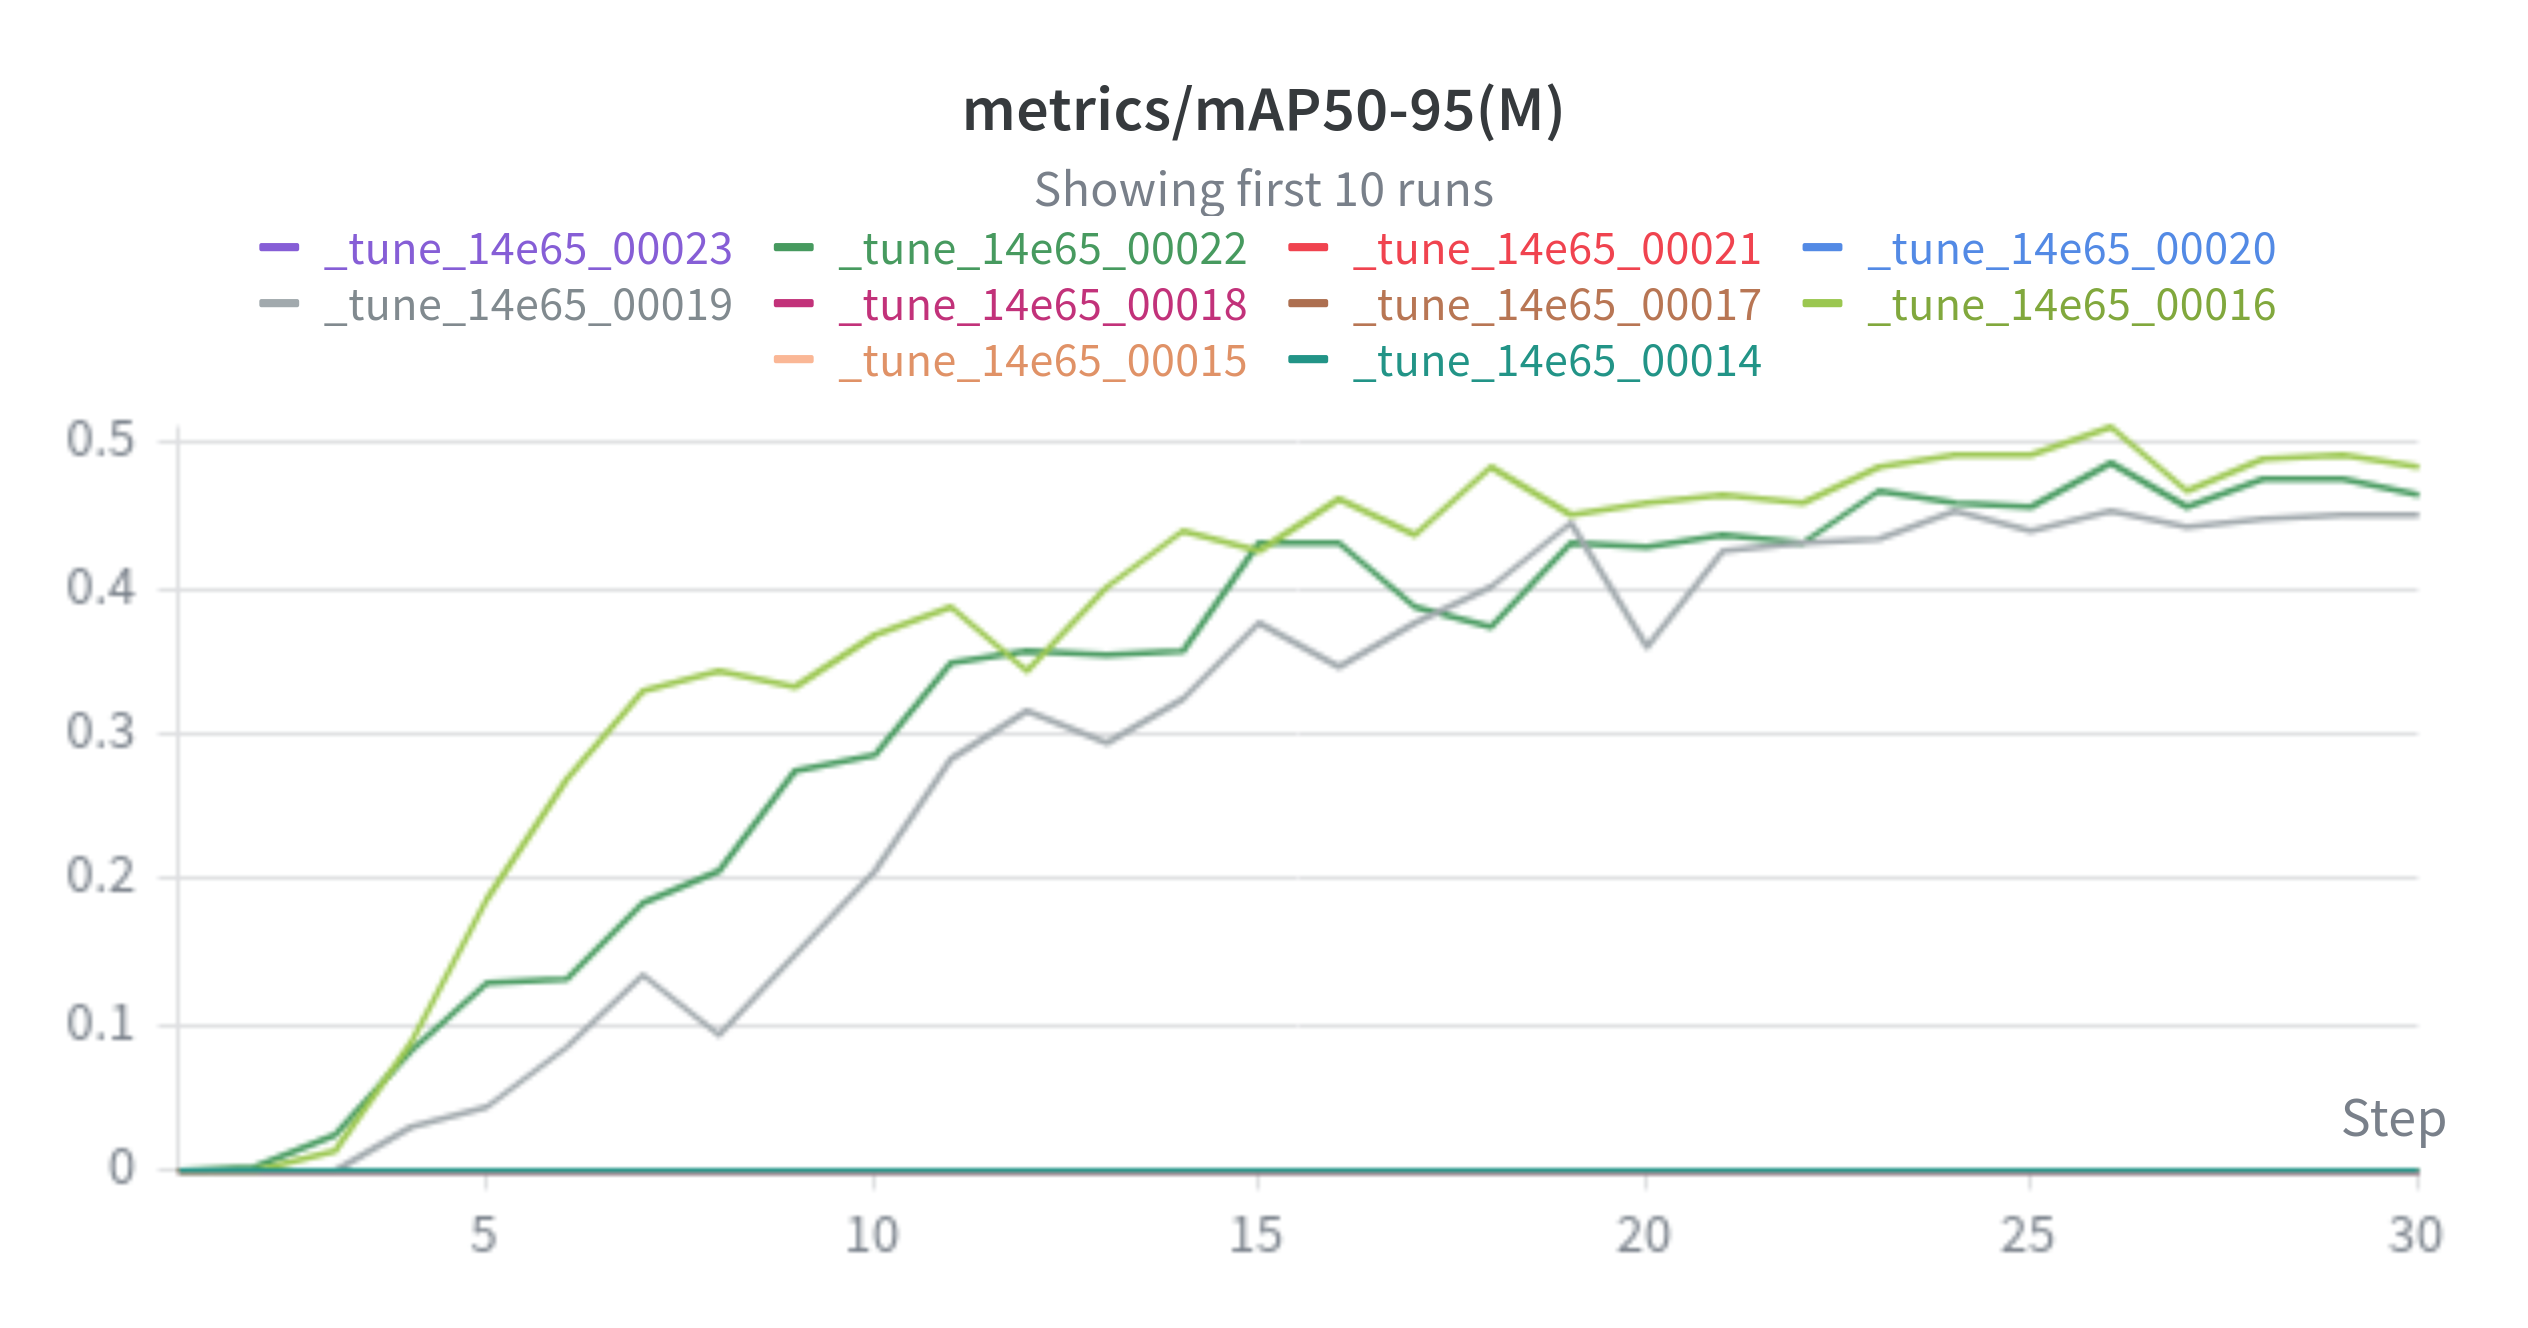
\includegraphics[width=0.82\textwidth]{figures/results/stage1_yolo_mAP50-95_M.png}
    \caption{Stage 1 validation mask $\mathrm{mAP}_{50\text{:}95}$ for the first ten runs shown in the \gls{wandb} sweep export. Only a small subset of configurations produced non-zero validation performance.}
    \label{fig:stage1_mask_map}
\end{figure}

The most relevant outcome of the tuning pipeline was that the best Stage 2
configuration consistently selected a batch size of 16 and an input resolution of
768 pixels. Stage 3 then resumed training from this configuration with a reduced
initial learning rate.

Figure~\ref{fig:stage2_mask_map} shows the broader Stage 2 validation mask
$\mathrm{mAP}_{50\text{:}95}$ trends. In contrast to Stage 1, Stage 2 produced a
larger number of usable configurations because the search was restricted to the
top Stage 1 candidates and only varied image size and batch size. The logged
results show that eight out of sixteen unique Stage 2 configurations achieved
non-zero mask $\mathrm{mAP}_{50\text{:}95}$ values. Most successful runs were
observed at an input resolution of 640 pixels, while many 768-pixel variants
remained unsuccessful. The main exception was the
\texttt{cfg1\_b16\_sz768} configuration, which produced the best Stage 2 result
and was therefore selected for Stage 3 refinement.

\begin{figure}[htbp]
    \centering
    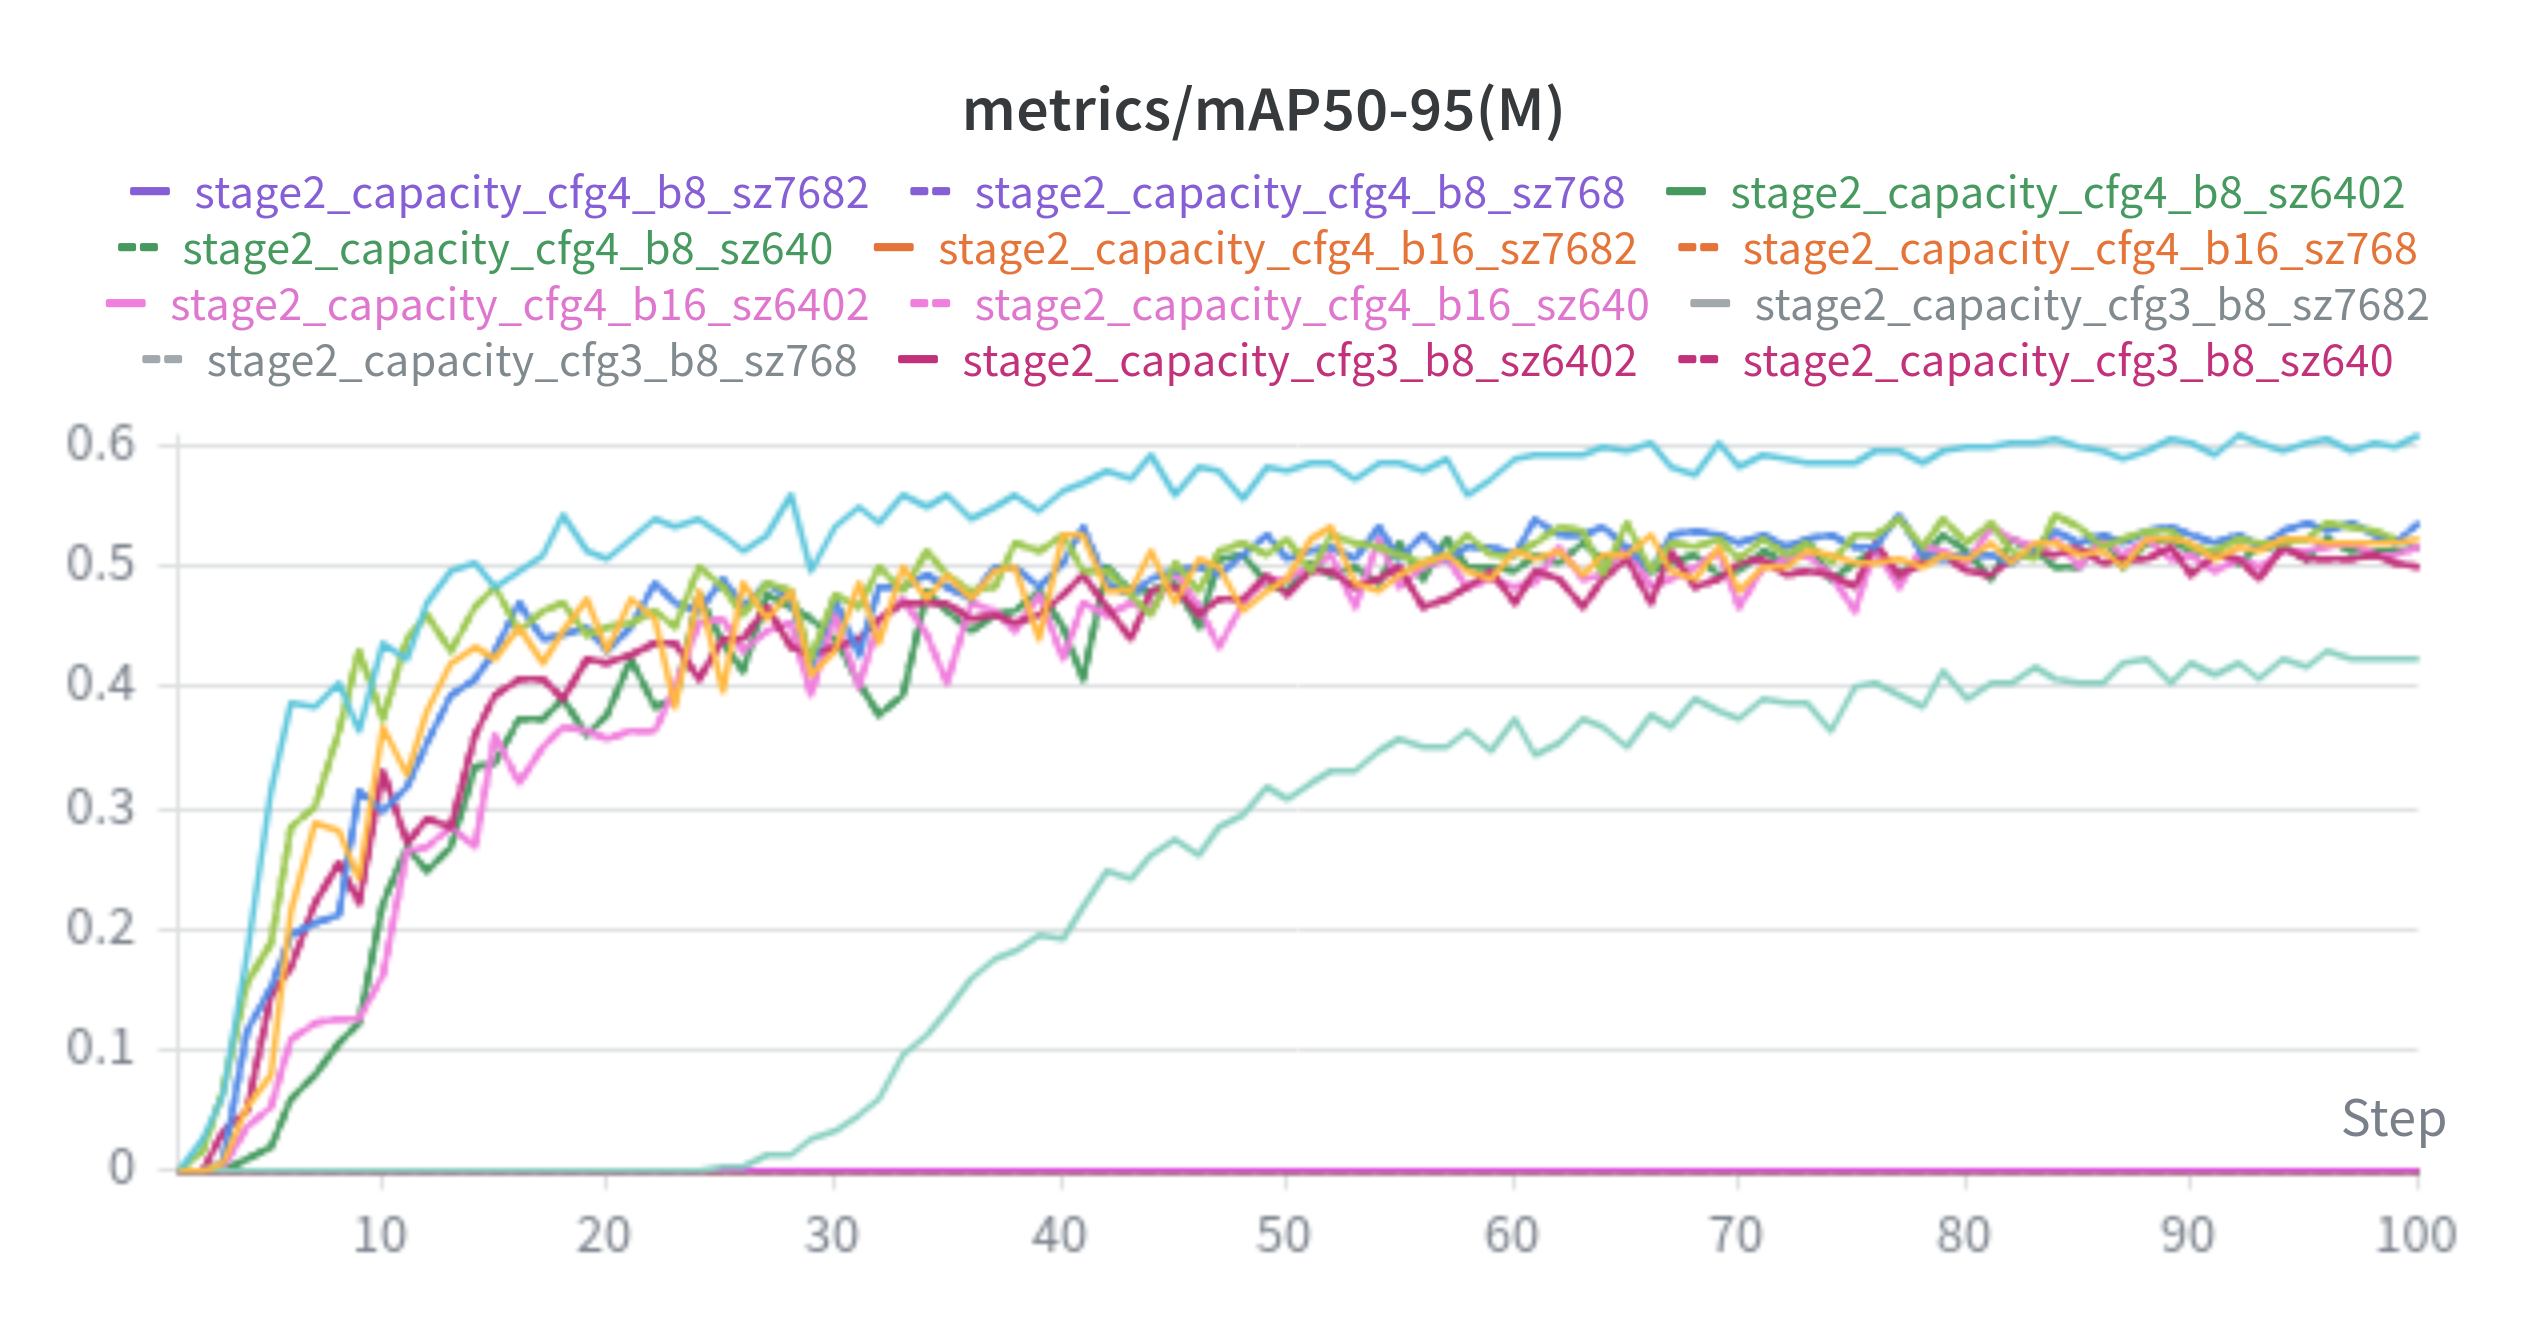
\includegraphics[width=0.82\textwidth]{figures/results/stage2_yolo_mAP50-95_m_full.png}
    \caption{Stage 2 validation mask $\mathrm{mAP}_{50\text{:}95}$ for the broader set of capacity-tuning runs. Compared with Stage 1, more configurations produced usable validation performance, although unsuccessful runs were still present.}
    \label{fig:stage2_mask_map}
\end{figure}

Table~\ref{tab:yolo_tuning_results} summarizes the best validation results of the
baseline model and the best Stage 3 tuned model. The tuned model reached its best
validation performance at epoch 120 and improved mask
$\mathrm{mAP}_{50\text{:}95}$ from 0.59645 to 0.63064. This corresponds to an absolute
gain of 0.03419 on the validation set. Precision changed only slightly, while
recall increased from 0.89947 to 0.90810, indicating that the tuned model mainly
benefited from better localization and mask quality rather than from a major shift
in confidence calibration. This improvement, however, should be interpreted as a
validation-stage model-selection result and not as evidence that the tuned model
outperformed the baseline on the final held-out test set.

Figures~\ref{fig:stage3_mask_map} and \ref{fig:stage3_val_seg_loss} show the
behavior of the two Stage 3 refinement runs. Both runs followed almost identical
validation trajectories, which indicates that the refinement step was stable once
the best Stage 2 configuration had been selected. The validation mask
$\mathrm{mAP}_{50\text{:}95}$ increased rapidly in the early epochs and then
stabilized slightly above 0.62. At the same time, the validation segmentation
loss dropped sharply at the start of training and then remained close to a stable
plateau. These curves indicate a controlled refinement of an already strong
configuration rather than a major qualitative change in optimization behavior.

\begin{figure}[htbp]
    \centering
    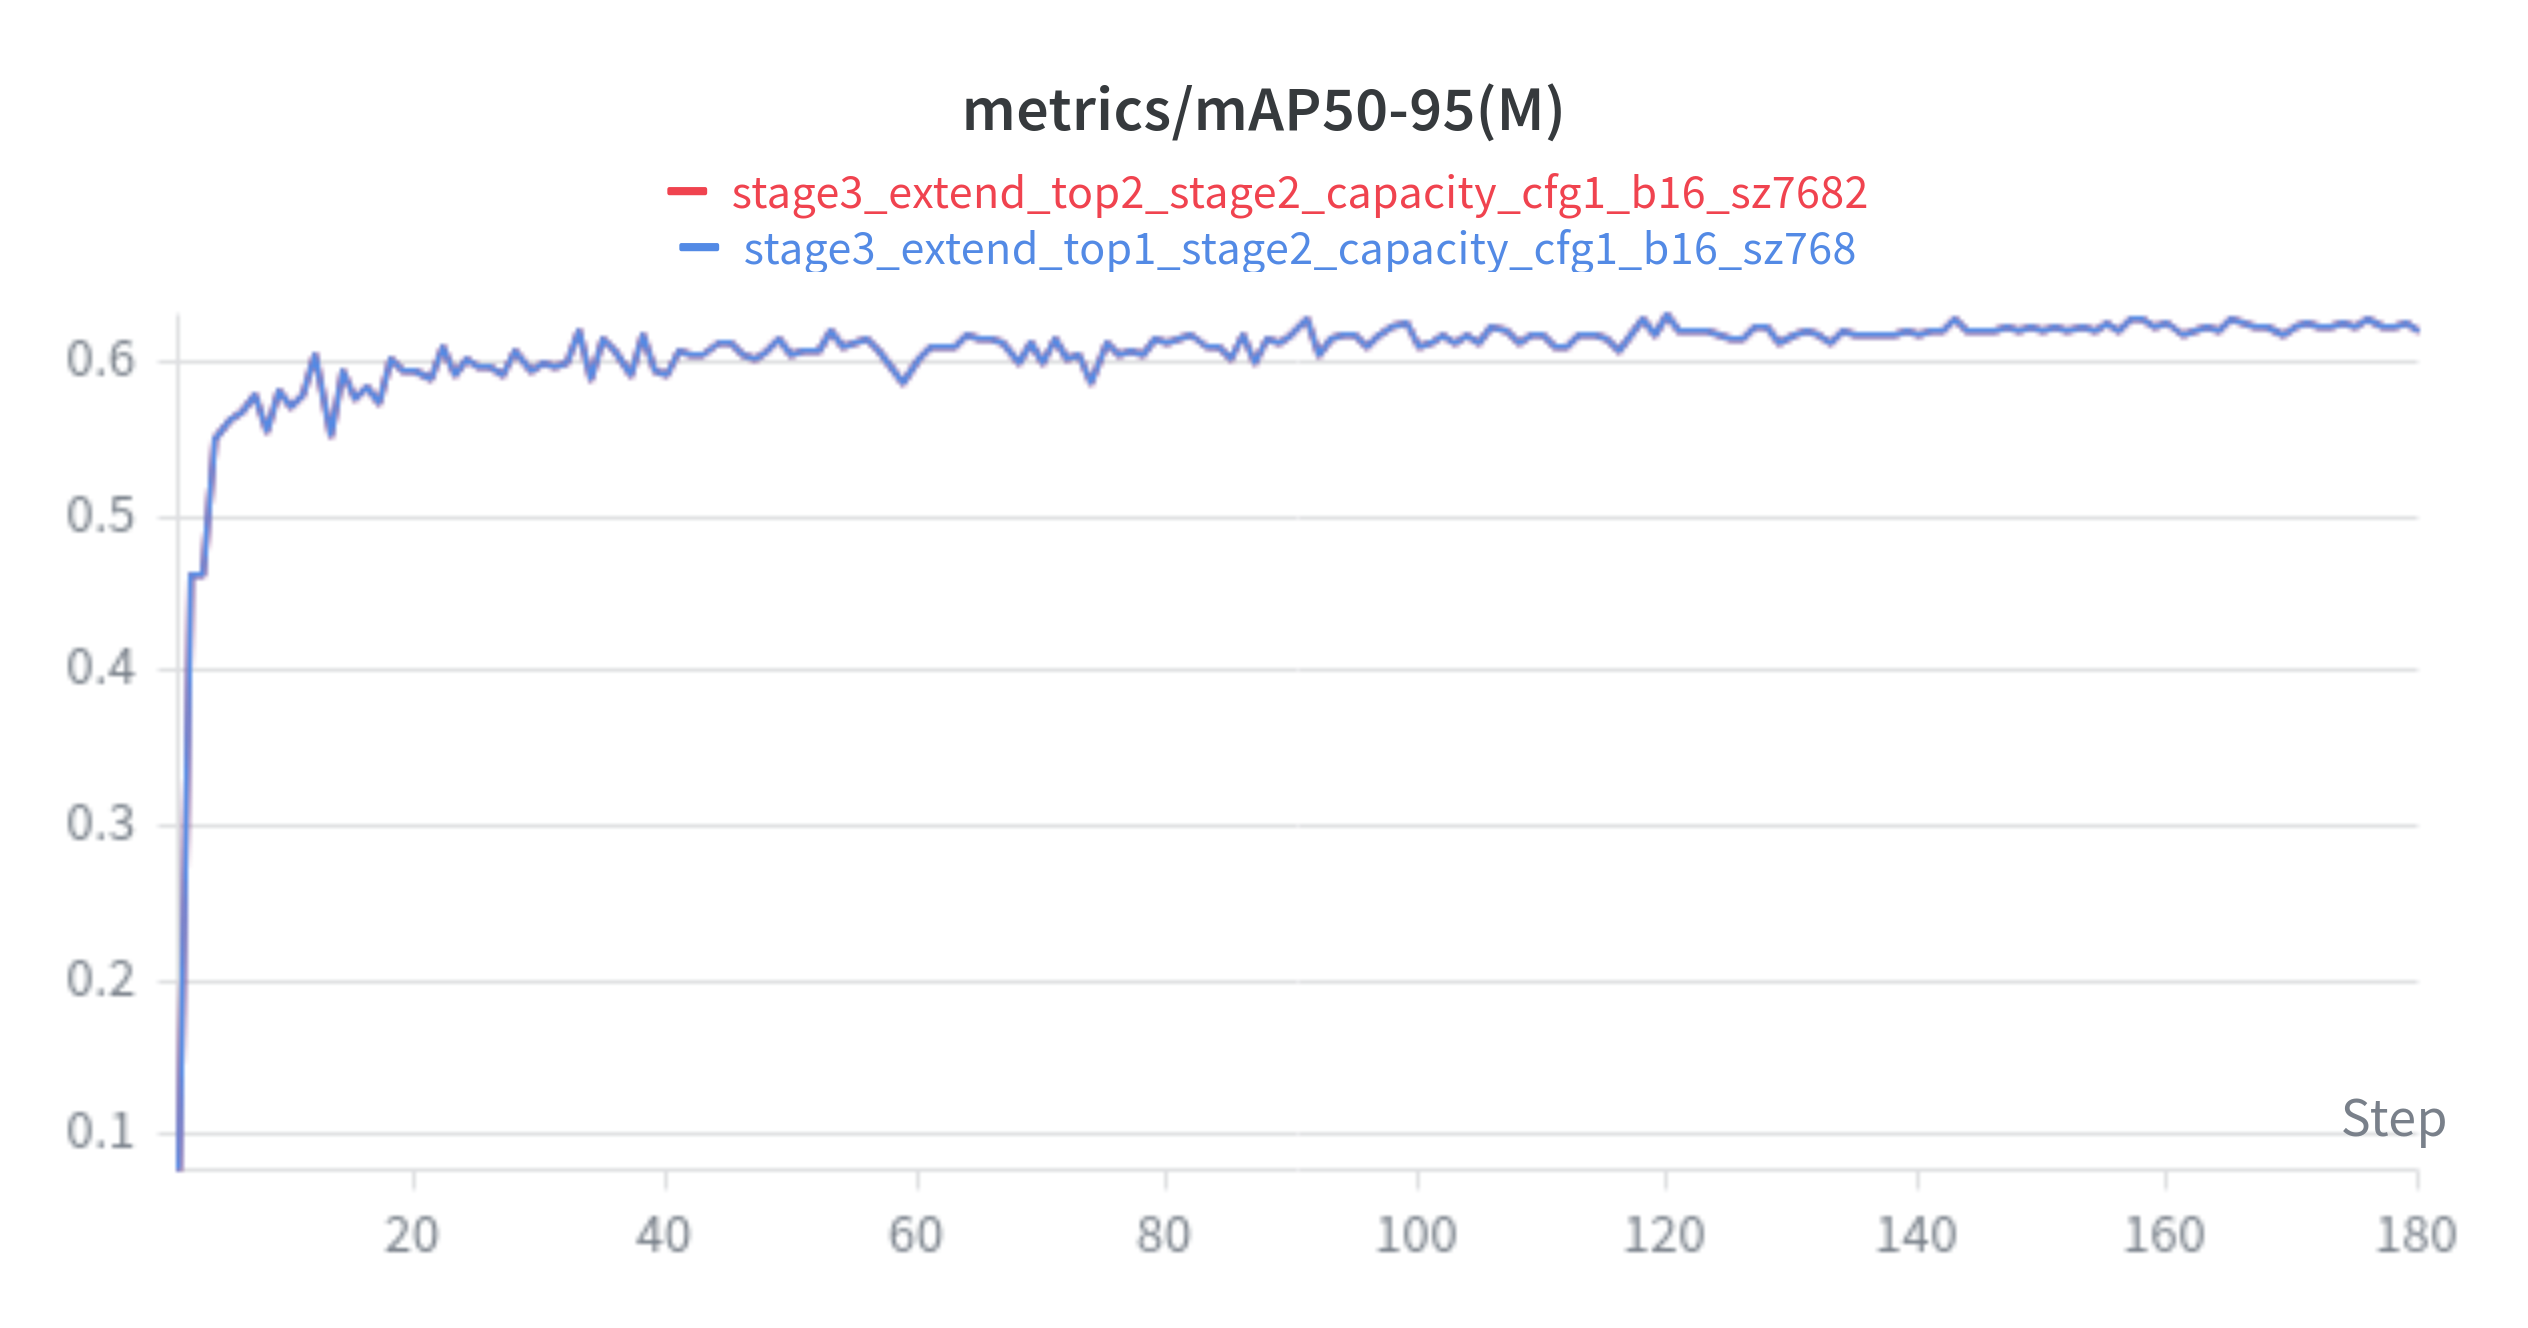
\includegraphics[width=0.82\textwidth]{figures/results/stage3_yolo_mAP50-95_M.png}
    \caption{Stage 3 validation mask $\mathrm{mAP}_{50\text{:}95}$ for the two refinement runs. The runs followed nearly identical trajectories and converged to the same performance region.}
    \label{fig:stage3_mask_map}
\end{figure}

\begin{figure}[htbp]
    \centering
    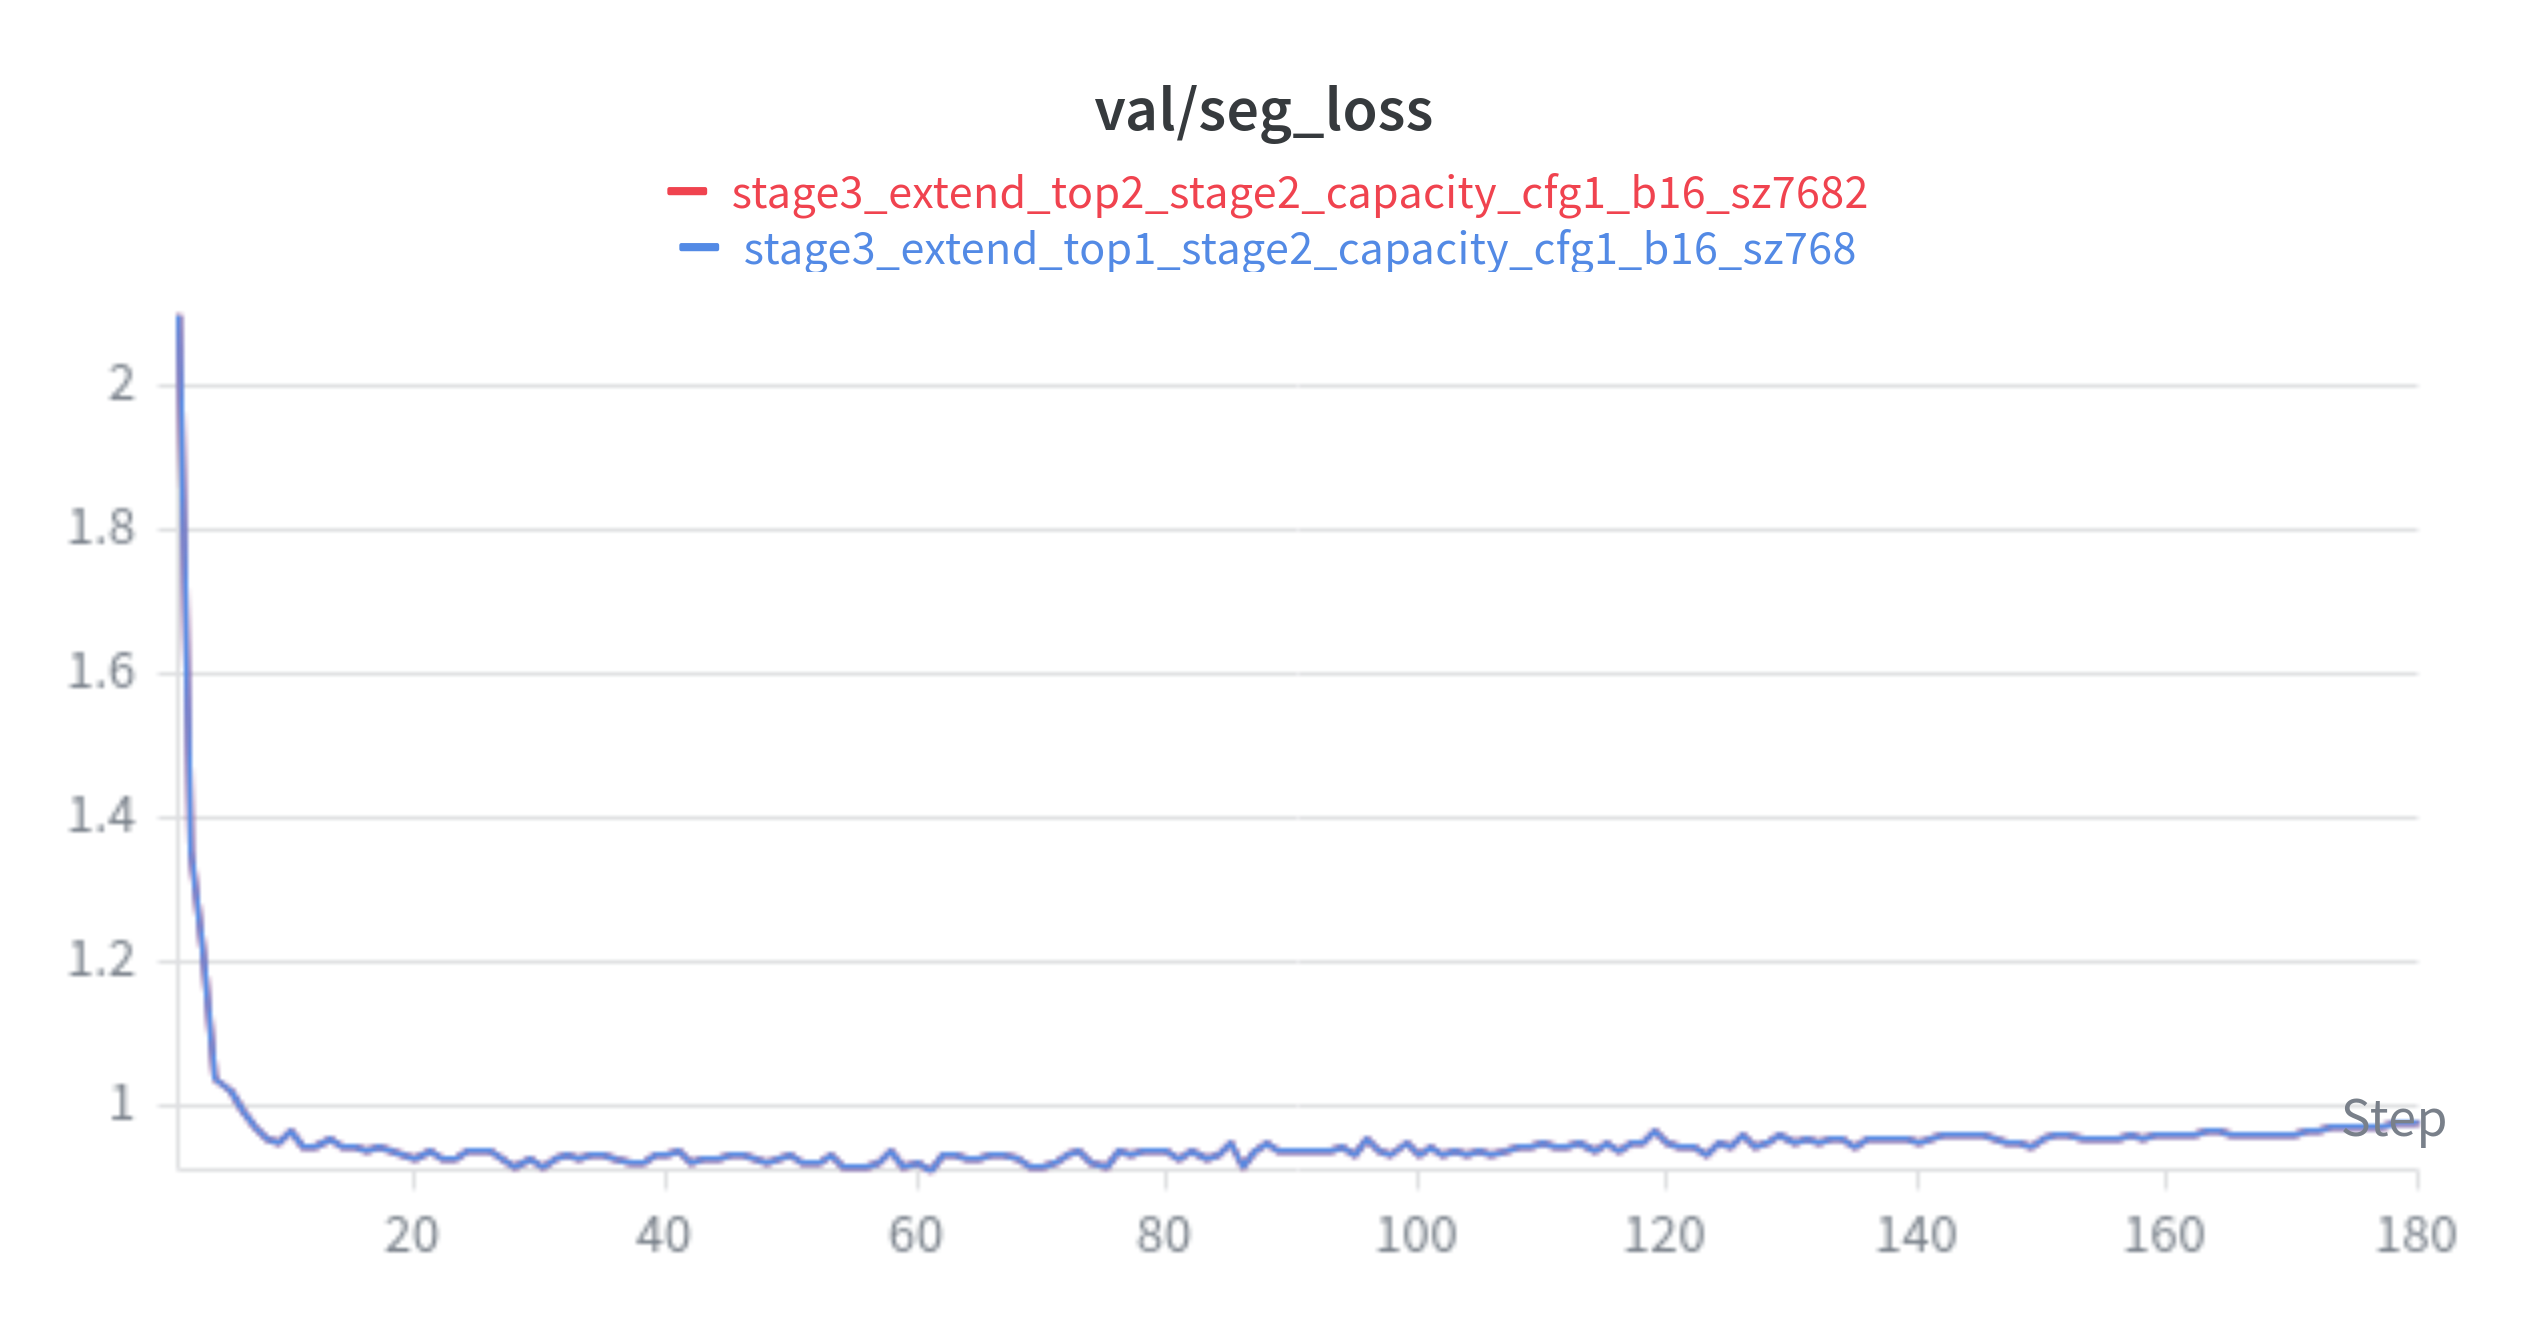
\includegraphics[width=0.82\textwidth]{figures/results/stage3_yolo_seg_loss_val.png}
    \caption{Stage 3 validation segmentation loss. After a steep initial decrease, the loss remained stable, indicating consistent convergence during refinement.}
    \label{fig:stage3_val_seg_loss}
\end{figure}

\begin{table}[htbp]
    \centering
    \caption{Best validation results of the baseline and tuned \gls{yolo}v8-Seg models.}
    \label{tab:yolo_tuning_results}
    \small
    \begin{tabular}{lccccc}
        \toprule
        Model & Best epoch & Mask $\mathrm{mAP}_{50}$ & Mask $\mathrm{mAP}_{50\text{:}95}$ & Mask precision & Mask recall \\
        \midrule
        Baseline YOLOv8-Seg & 49 & 0.93931 & 0.59645 & 0.90623 & 0.89947 \\
        Stage 3 tuned YOLOv8-Seg & 120 & 0.94268 & 0.63064 & 0.90150 & 0.90810 \\
        \bottomrule
    \end{tabular}
\end{table}

\begin{table}[htbp]
    \centering
    \caption{Held-out test-set comparison between the baseline and the selected Stage 3 tuned \gls{yolo}v8-Seg model.}
    \label{tab:yolo_tuning_test_results}
    \small
    \begin{tabular}{lccccc}
        \toprule
        Model & Image size & Mask $\mathrm{mAP}_{50}$ & Mask $\mathrm{mAP}_{50\text{:}95}$ & Mask precision & Mask recall \\
        \midrule
        Baseline YOLOv8-Seg & 640 & 0.92819 & 0.73744 & 0.87603 & 0.90832 \\
        Stage 3 tuned YOLOv8-Seg & 640 & 0.91706 & 0.68829 & 0.86839 & 0.88443 \\
        Baseline YOLOv8-Seg & 768 & 0.92638 & 0.74752 & 0.86778 & 0.92329 \\
        Stage 3 tuned YOLOv8-Seg & 768 & 0.92719 & 0.71985 & 0.87399 & 0.90724 \\
        \bottomrule
    \end{tabular}
\end{table}

These results show that systematic hyperparameter tuning was useful for improving
validation performance. However, the held-out test comparison in
Table~\ref{tab:yolo_tuning_test_results} does not support replacing the baseline
checkpoint with the Stage 3 model. At an image size of 640 pixels, the baseline
outperformed the tuned model by 0.04915 mask $\mathrm{mAP}_{50\text{:}95}$, and
at 768 pixels the margin remained 0.02767 in favor of the baseline. For this
reason, the original baseline checkpoint remained the reference model for the
later deployment-oriented experiments and for the final adaptation study.

\subsection{Comparison with YOLO26}

To evaluate whether a newer Ultralytics architecture could provide a better
segmentation model under comparable conditions, YOLO26-small was trained using
the same baseline recipe and later extended to a longer 180-epoch run. The final
comparison was performed on the held-out original test split at image sizes of 640
and 768 pixels.

The results are presented in Table~\ref{tab:yolo26_comparison}. At an image size
of 640 pixels, the baseline \gls{yolo}v8-Seg model achieved a mask
$\mathrm{mAP}_{50\text{:}95}$ of 0.58295, whereas YOLO26 reached 0.57538. At 768
pixels, the baseline again remained slightly better, with 0.62325 compared with
0.61689 for YOLO26. The higher-resolution evaluation benefited both models, but it
did not change the ranking between them. Under the training and evaluation
conditions used in this project, YOLO26 therefore did not outperform the baseline
\gls{yolo}v8-Seg model on the held-out test set.

Figure~\ref{fig:yolo26_mask_map} shows the corresponding validation mask
$\mathrm{mAP}_{50\text{:}95}$ curves for the two YOLO26 runs. Extending the
training to 180 epochs shifted the validation curve upward and produced a higher
plateau than the shorter run. However, the improvement remained modest and was
not sufficient to reverse the final test-set ranking against the baseline
\gls{yolo}v8-Seg model.

\begin{table}[htbp]
    \centering
    \caption{Test-set comparison between the baseline \gls{yolo}v8-Seg model and YOLO26-small.}
    \label{tab:yolo26_comparison}
    \small
    \begin{tabular}{lccccc}
        \toprule
        Model & Image size & Mask $\mathrm{mAP}_{50}$ & Mask $\mathrm{mAP}_{50\text{:}95}$ & Mask precision & Mask recall \\
        \midrule
        YOLOv8-Seg baseline & 640 & 0.91921 & 0.58295 & 0.86835 & 0.89896 \\
        YOLO26-small & 640 & 0.91209 & 0.57538 & 0.87300 & 0.89879 \\
        YOLOv8-Seg baseline & 768 & 0.92384 & 0.62325 & 0.86577 & 0.91939 \\
        YOLO26-small & 768 & 0.92596 & 0.61689 & 0.88408 & 0.91326 \\
        \bottomrule
    \end{tabular}
\end{table}

\begin{figure}[htbp]
    \centering
    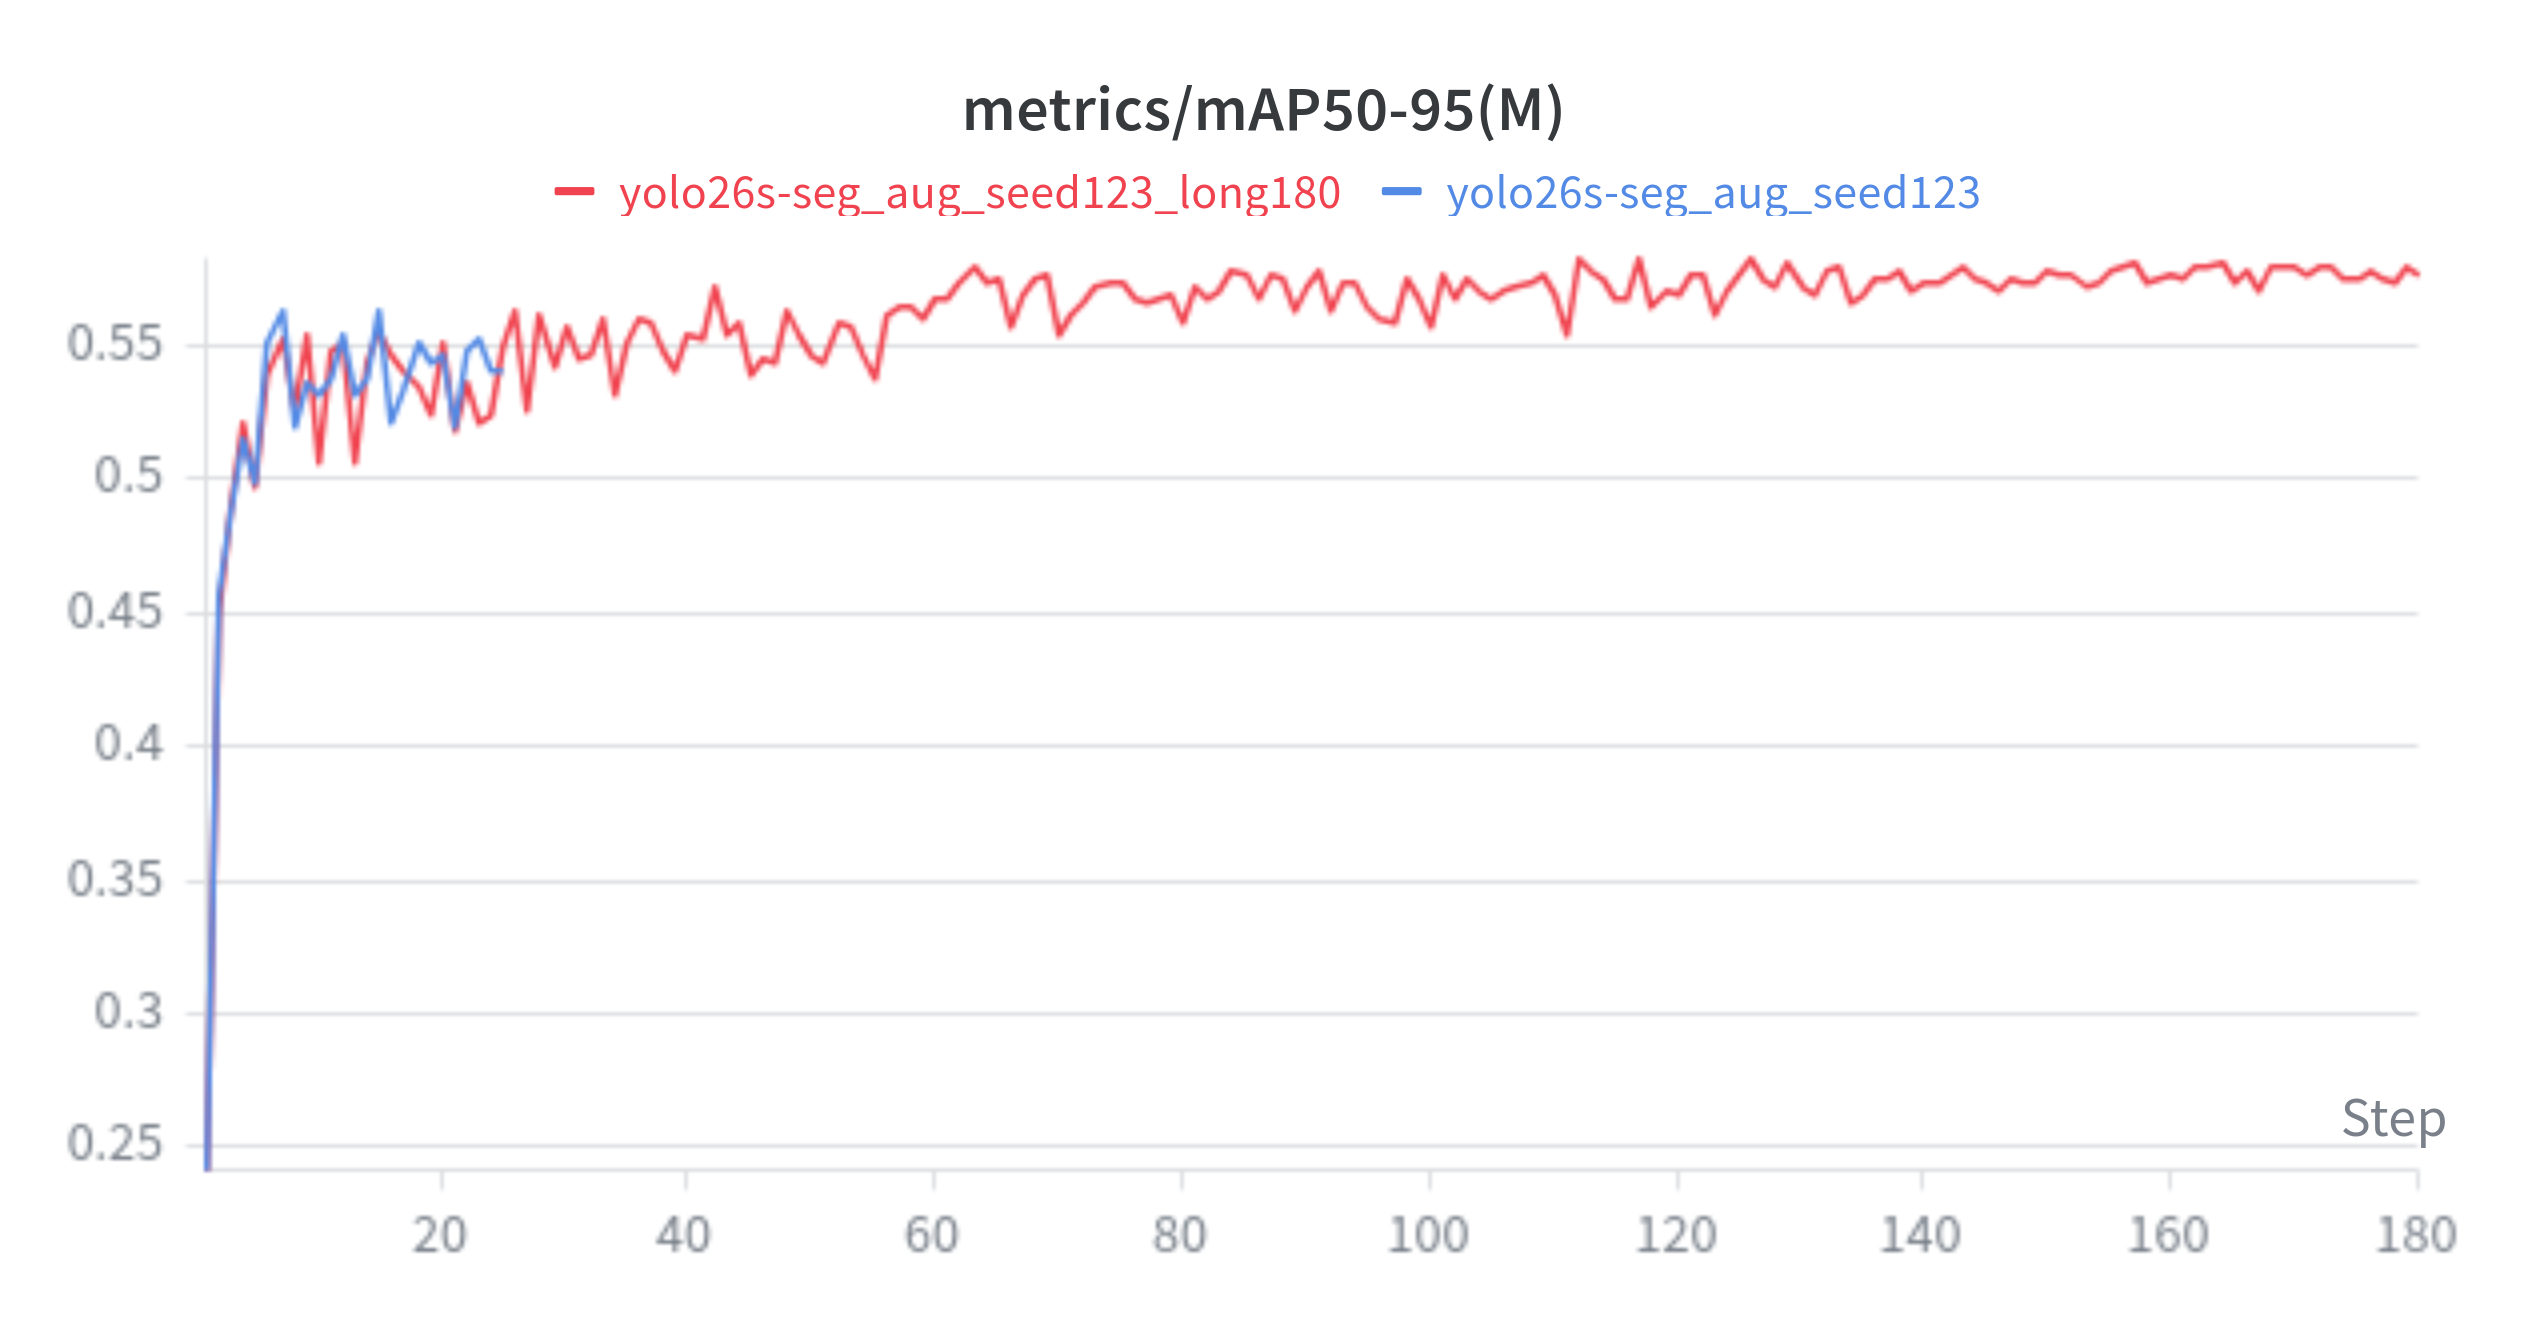
\includegraphics[width=0.82\textwidth]{figures/results/yolo26_mAP50-95_M.png}
    \caption{Validation mask $\mathrm{mAP}_{50\text{:}95}$ for the two YOLO26 training runs. The longer 180-epoch run improved over the shorter run, but the resulting model still did not surpass the YOLOv8 baseline on the held-out test set.}
    \label{fig:yolo26_mask_map}
\end{figure}

\subsection{Environment-specific fine-tuning with \gls{adc} data}

The final \gls{yolo} experiment focused on adaptation to the target university
environment. For this purpose, the baseline checkpoint was fine-tuned on a mixed
dataset that combined the original elevator-panel dataset with 46 newly
collected and annotated images from HAN University, Building 31. This building
served as the pilot environment for planned robot deployment tests. The
environment-specific images were collected with the \gls{adc} and then split into
32 training images, 7 validation images, and 7 test images before being merged
with the original dataset. The resulting evaluation therefore makes it possible
to determine whether the adapted model improves in the target environment without
losing too much performance on the original domain.

Table~\ref{tab:adc_original_test} shows the results on the original held-out test
split. The fine-tuned model remained effectively tied with the baseline. Its mask
$\mathrm{mAP}_{50\text{:}95}$ changed from 0.58295 to 0.58293, which is
negligible. The box metrics improved slightly, and mask precision and recall also
increased marginally. This indicates that adaptation to the new environment did
not cause a meaningful degradation on the original dataset.

The corresponding validation curve is shown in
Figure~\ref{fig:adc_finetune_mask_map}. The fine-tuned model remained in the same
overall validation range as the original baseline, with modest fluctuations
around 0.58. This is consistent with the final original-test comparison, which
showed that the fine-tuned model preserved the baseline's general performance
while becoming substantially more effective on the environment-specific
\texttt{adc\_first} test set.

\begin{table}[htbp]
    \centering
    \caption{Performance on the original held-out elevator test split before and after \gls{adc} fine-tuning.}
    \label{tab:adc_original_test}
    \small
    \begin{tabular}{lcccc}
        \toprule
        Model & Mask $\mathrm{mAP}_{50}$ & Mask $\mathrm{mAP}_{50\text{:}95}$ & Mask precision & Mask recall \\
        \midrule
        Baseline YOLOv8-Seg & 0.91921 & 0.58295 & 0.86835 & 0.89896 \\
        \glsentryshort{adc} fine-tuned YOLOv8-Seg & 0.91912 & 0.58293 & 0.88043 & 0.90050 \\
        \bottomrule
    \end{tabular}
\end{table}

\begin{figure}[htbp]
    \centering
    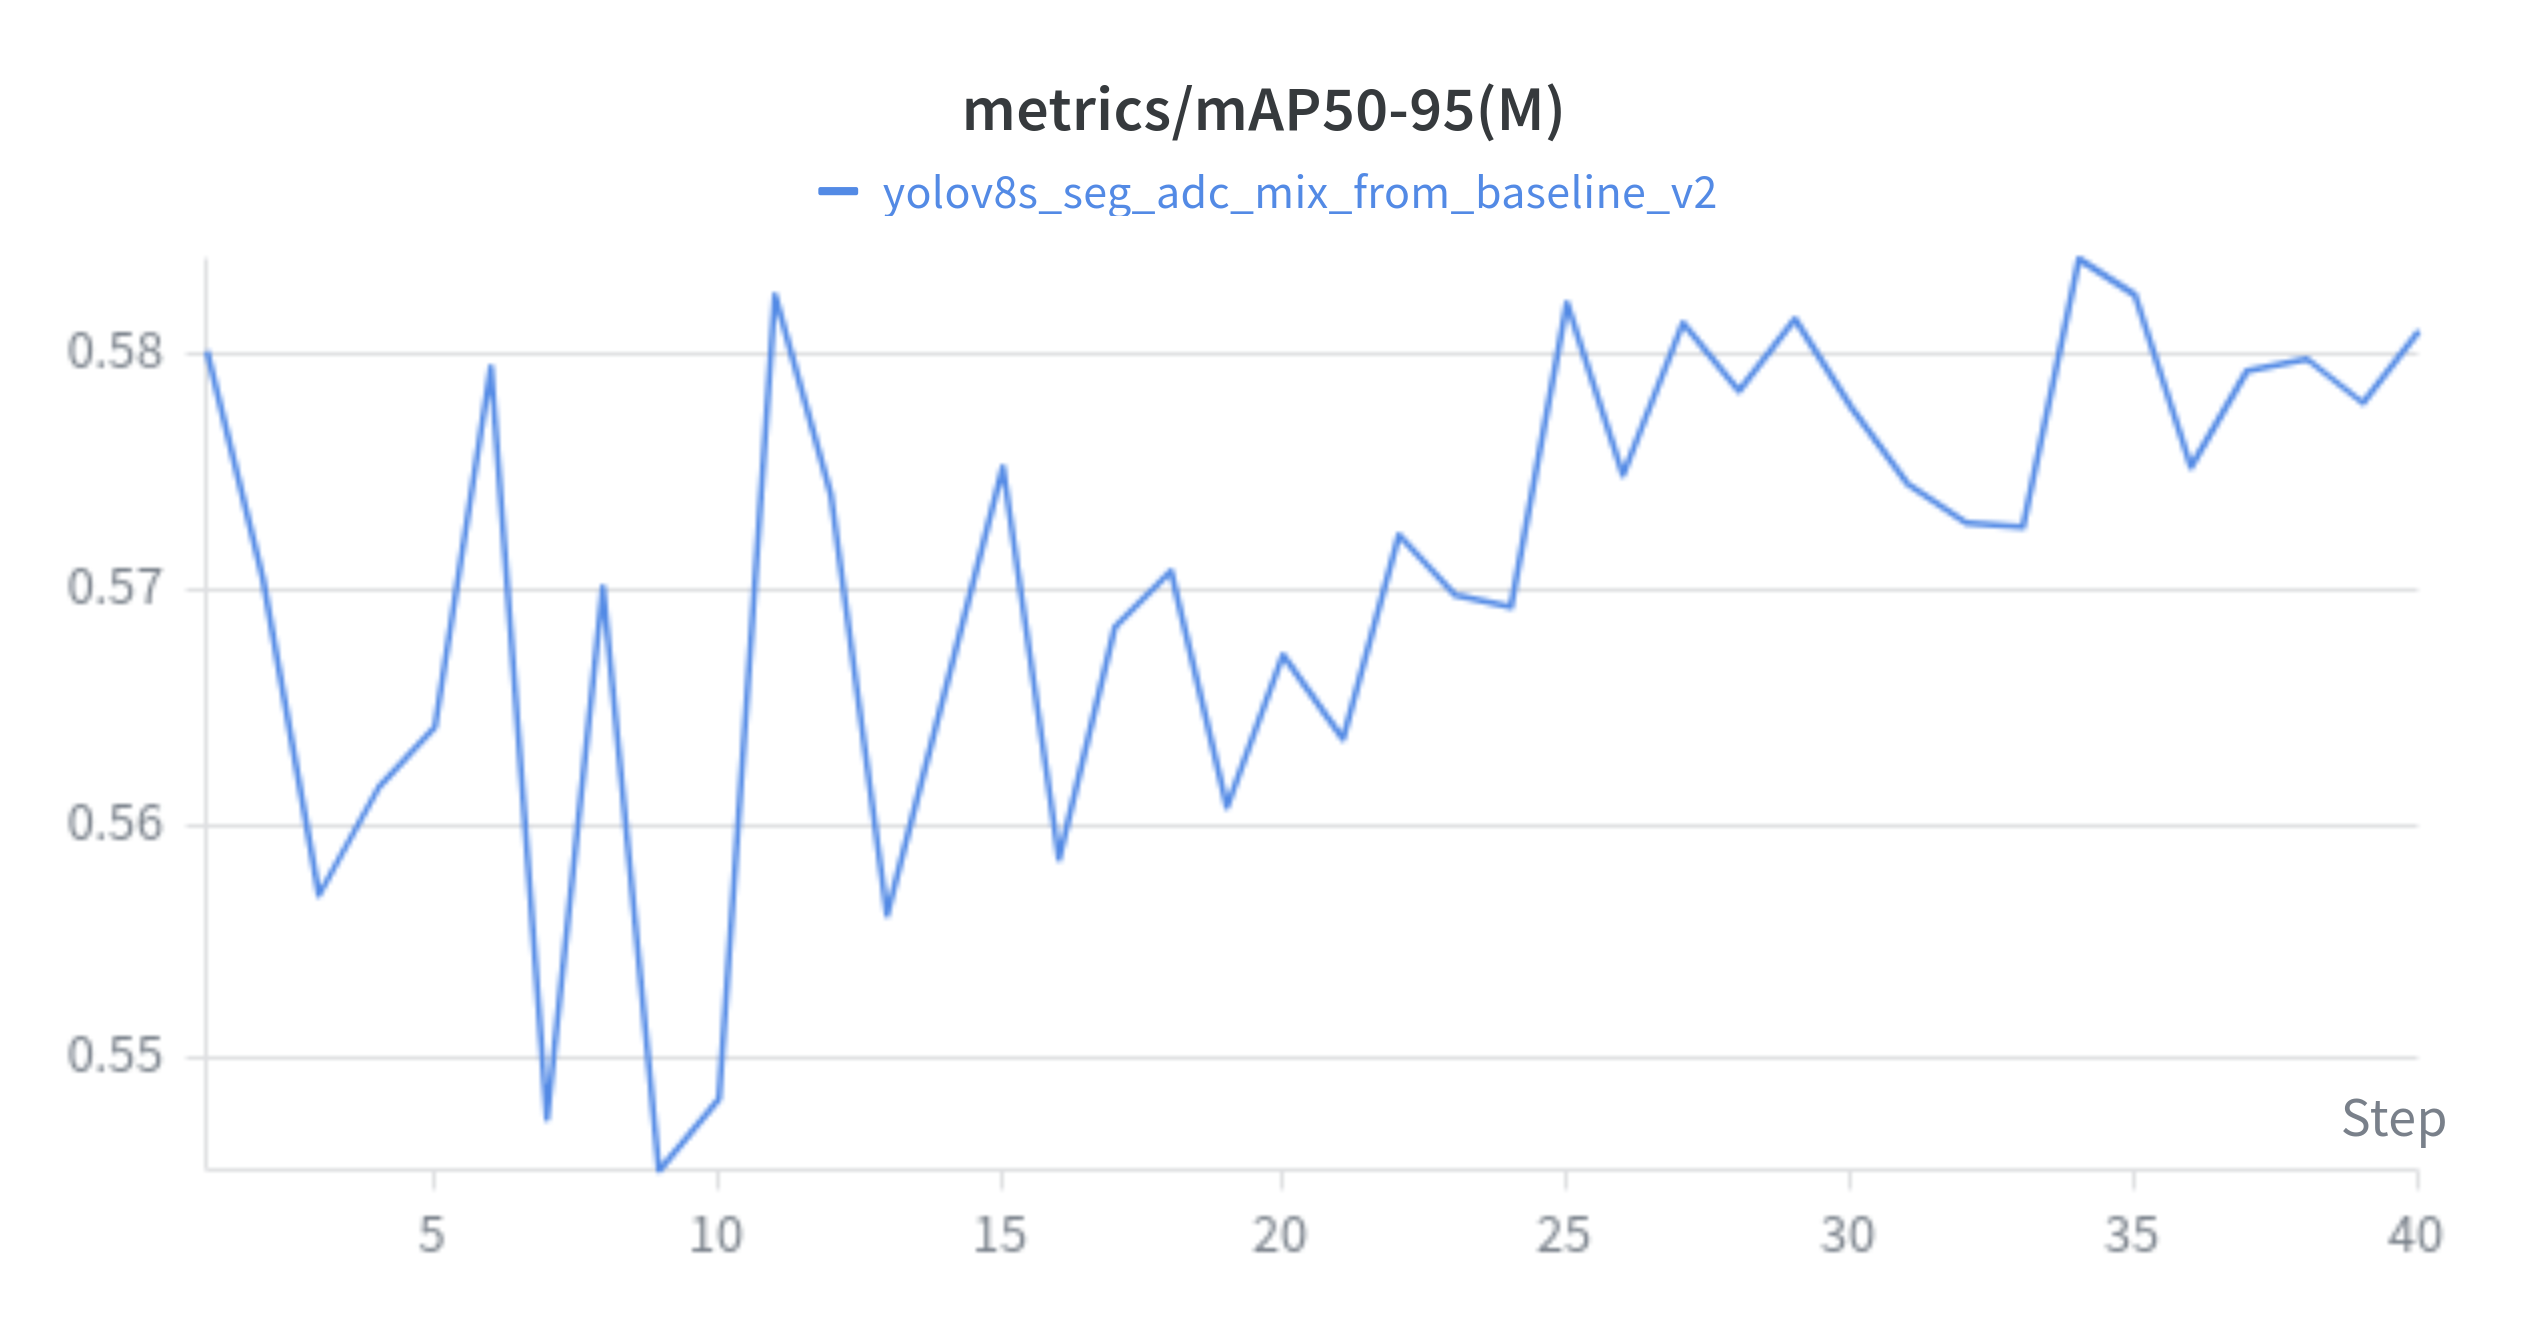
\includegraphics[width=0.82\textwidth]{figures/results/yolo_adc_fine_tune_mAP50-95_M.png}
    \caption{Validation mask $\mathrm{mAP}_{50\text{:}95}$ during \gls{adc}-based fine-tuning. The curve remains close to the baseline validation range, which aligns with the near-identical performance observed on the original held-out test split.}
    \label{fig:adc_finetune_mask_map}
\end{figure}

The effect on the \gls{adc}-specific test set is much more pronounced, as shown in
Table~\ref{tab:adc_env_test}. On this environment-specific split, the baseline
model achieved a mask $\mathrm{mAP}_{50\text{:}95}$ of only 0.12290. After
fine-tuning, the same metric increased to 0.50463. Mask precision increased from
0.61209 to 1.00000, and mask recall increased from 0.70136 to 0.99712. This is
the clearest result of the \gls{yolo} experiments: collecting a relatively small
amount of real deployment data and using it for controlled fine-tuning
substantially improved performance in the target environment while preserving the
performance level on the original test set.

\begin{table}[htbp]
    \centering
    \caption{Performance on the environment-specific \gls{adc} test split before and after \gls{adc} fine-tuning.}
    \label{tab:adc_env_test}
    \small
    \begin{tabular}{lcccc}
        \toprule
        Model & Mask $\mathrm{mAP}_{50}$ & Mask $\mathrm{mAP}_{50\text{:}95}$ & Mask precision & Mask recall \\
        \midrule
        Baseline YOLOv8-Seg & 0.53520 & 0.12290 & 0.61209 & 0.70136 \\
        \glsentryshort{adc} fine-tuned YOLOv8-Seg & 0.99500 & 0.50463 & 1.00000 & 0.99712 \\
        \bottomrule
    \end{tabular}
\end{table}

This environment-specific improvement was also reflected in deployment-oriented
behavior after retraining on \gls{adc} data from HAN University, Building 31.
In a controlled replay experiment on the same recorded \gls{rgbd} sequence, the
retrained model increased mean target confidence from 0.8184 to 0.8422 and
raised the 10th-percentile target confidence from 0.6562 to 0.7727, indicating
that the main gain occurred in weaker detections rather than only in already
easy cases. Distance-related improvements were more scenario-dependent, but live
deployment observations showed a practical increase in outside elevator-panel
single-button recognition distance from approximately 35~cm to 75~cm. This
distance gain should be interpreted as a task-specific field observation rather
than a universal range increase across all scenes, but it still supports the
conclusion that retraining improved practical usability in the target building.

Overall, the \gls{yolo} results show three main findings. First, the baseline
\gls{yolo}v8-Seg model was already strong and difficult to surpass on the general
elevator test set. Second, staged hyperparameter tuning improved validation
performance but did not fundamentally change the final model ranking. Third, the
most practically valuable improvement was achieved through environment-specific
fine-tuning with \gls{adc} data, which substantially increased performance on the
target deployment domain while preserving performance on the original dataset.

\section{\Gls{ocr} hyperparameter tuning and evaluation}

The \gls{ocr} experiments focused on improving cropped-button recognition while keeping
the recognizer lightweight enough for later embedded deployment. As in the
\gls{yolo} experiments, model selection during \gls{ocr} tuning was based on the
validation split, and the final comparison between \gls{ocr} candidates was performed on
the held-out \gls{ocr} test set.

\subsection{Stage 1: epoch selection}

The first \gls{ocr} tuning stage varied only the number of training epochs while keeping
the optimizer configuration fixed. The main objective of this stage was to
determine whether the original 60-epoch fine-tuning recipe was necessary or
whether a shorter training budget would already achieve the same validation
quality.

Table~\ref{tab:ocr_stage1_results} shows that the 50-epoch and 60-epoch runs
converged to almost identical validation performance, both reaching their best
result at epoch 46. In contrast, the 30-epoch run underperformed clearly. This
indicates that the recognizer required more than 30 epochs to converge, but that
training beyond 50 epochs provided no meaningful additional benefit. For that
reason, 50 epochs were selected as the fixed budget for the next stage of \gls{ocr}
hyperparameter tuning. This interpretation is also supported by the Stage 1
training-loss curves shown in Figure~\ref{fig:ocr_stage1_loss}, where the main
decrease occurs well before the end of the 50-epoch run and the longer schedule
does not suggest a qualitatively different convergence regime.

\begin{figure}[htbp]
    \centering
    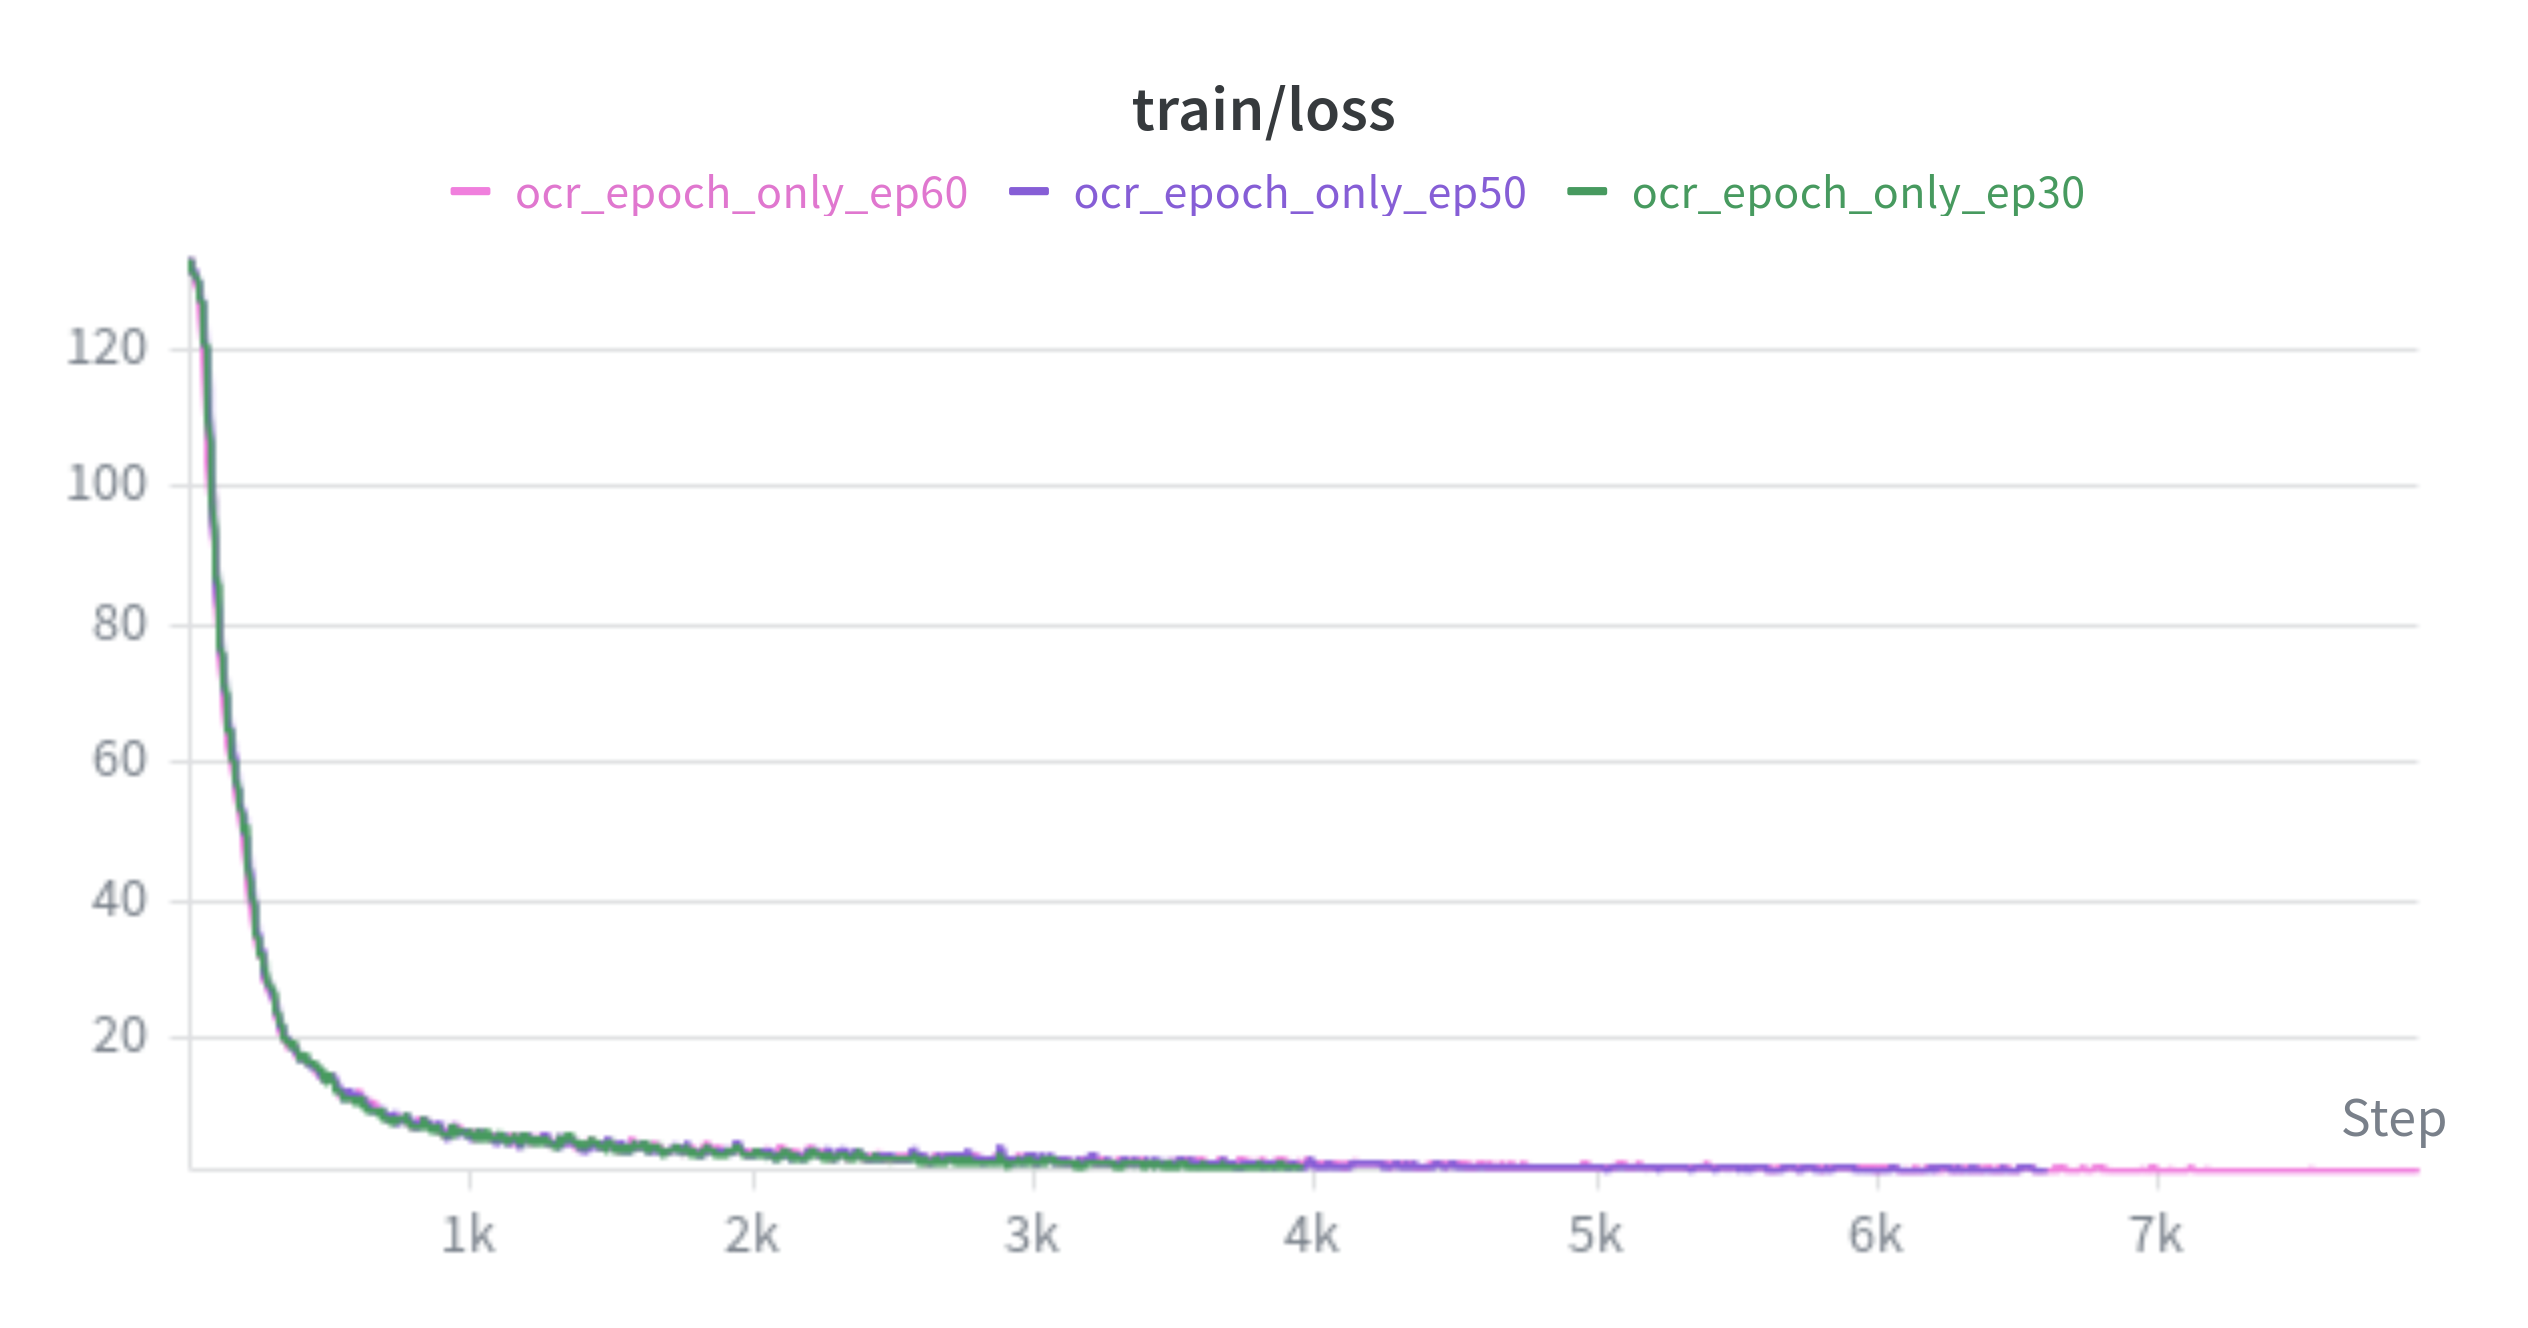
\includegraphics[width=0.82\textwidth]{figures/results/stage1_ocr_train_loss.png}
    \caption{Stage 1 \gls{ocr} training loss for the epoch-selection runs. Most of the
    optimization progress occurs before the 50-epoch mark, which supports the
    decision to use 50 epochs for the subsequent optimizer sweep.}
    \label{fig:ocr_stage1_loss}
\end{figure}

\begin{table}[htbp]
    \centering
    \caption{Stage 1 \gls{ocr} epoch-sweep results on the validation split.}
    \label{tab:ocr_stage1_results}
    \small
    \begin{tabular}{lccc}
        \toprule
        Trial & Best epoch & Accuracy & Normalized edit distance \\
        \midrule
        30 epochs & 16 & 0.78776 & 0.83732 \\
        50 epochs & 46 & 0.84124 & 0.87080 \\
        60 epochs & 46 & 0.84057 & 0.86893 \\
        \bottomrule
    \end{tabular}
\end{table}

\subsection{Stage 2: learning rate and weight decay sweep}

After fixing the training budget at 50 epochs, a second tuning stage evaluated a
narrow optimizer sweep over learning rate and weight decay. Four configurations
were tested. The resulting validation scores are summarized in
Table~\ref{tab:ocr_stage2_results}.

The best configuration used an initial learning rate of
$3 \times 10^{-4}$ and a weight decay of $3 \times 10^{-5}$. This run achieved a
validation accuracy of 0.84157 and a normalized edit distance of 0.87098, making
it the strongest \gls{ocr} candidate of the sweep. The configuration with the same
learning rate but lower weight decay performed substantially worse, while the run
using $5 \times 10^{-4}$ degraded sharply and converged to a much lower
performance level. Increasing the learning rate further to $7 \times 10^{-4}$
recovered most of the performance, but still remained below the best
$3 \times 10^{-4}$ run.

These results indicate that \gls{ocr} fine-tuning was sensitive to the optimizer
settings even within a relatively narrow search range. In particular, the stage-2
results suggest that a slightly lower learning rate than the original baseline
provided more stable and ultimately better convergence on the recognition task.
This behavior is visible in Figure~\ref{fig:ocr_stage2_acc}, where the best run
maintains the highest evaluation accuracy, and in
Figure~\ref{fig:ocr_stage2_ned}, where the same configuration also produces the
strongest normalized edit-distance curve.

\begin{figure}[htbp]
    \centering
    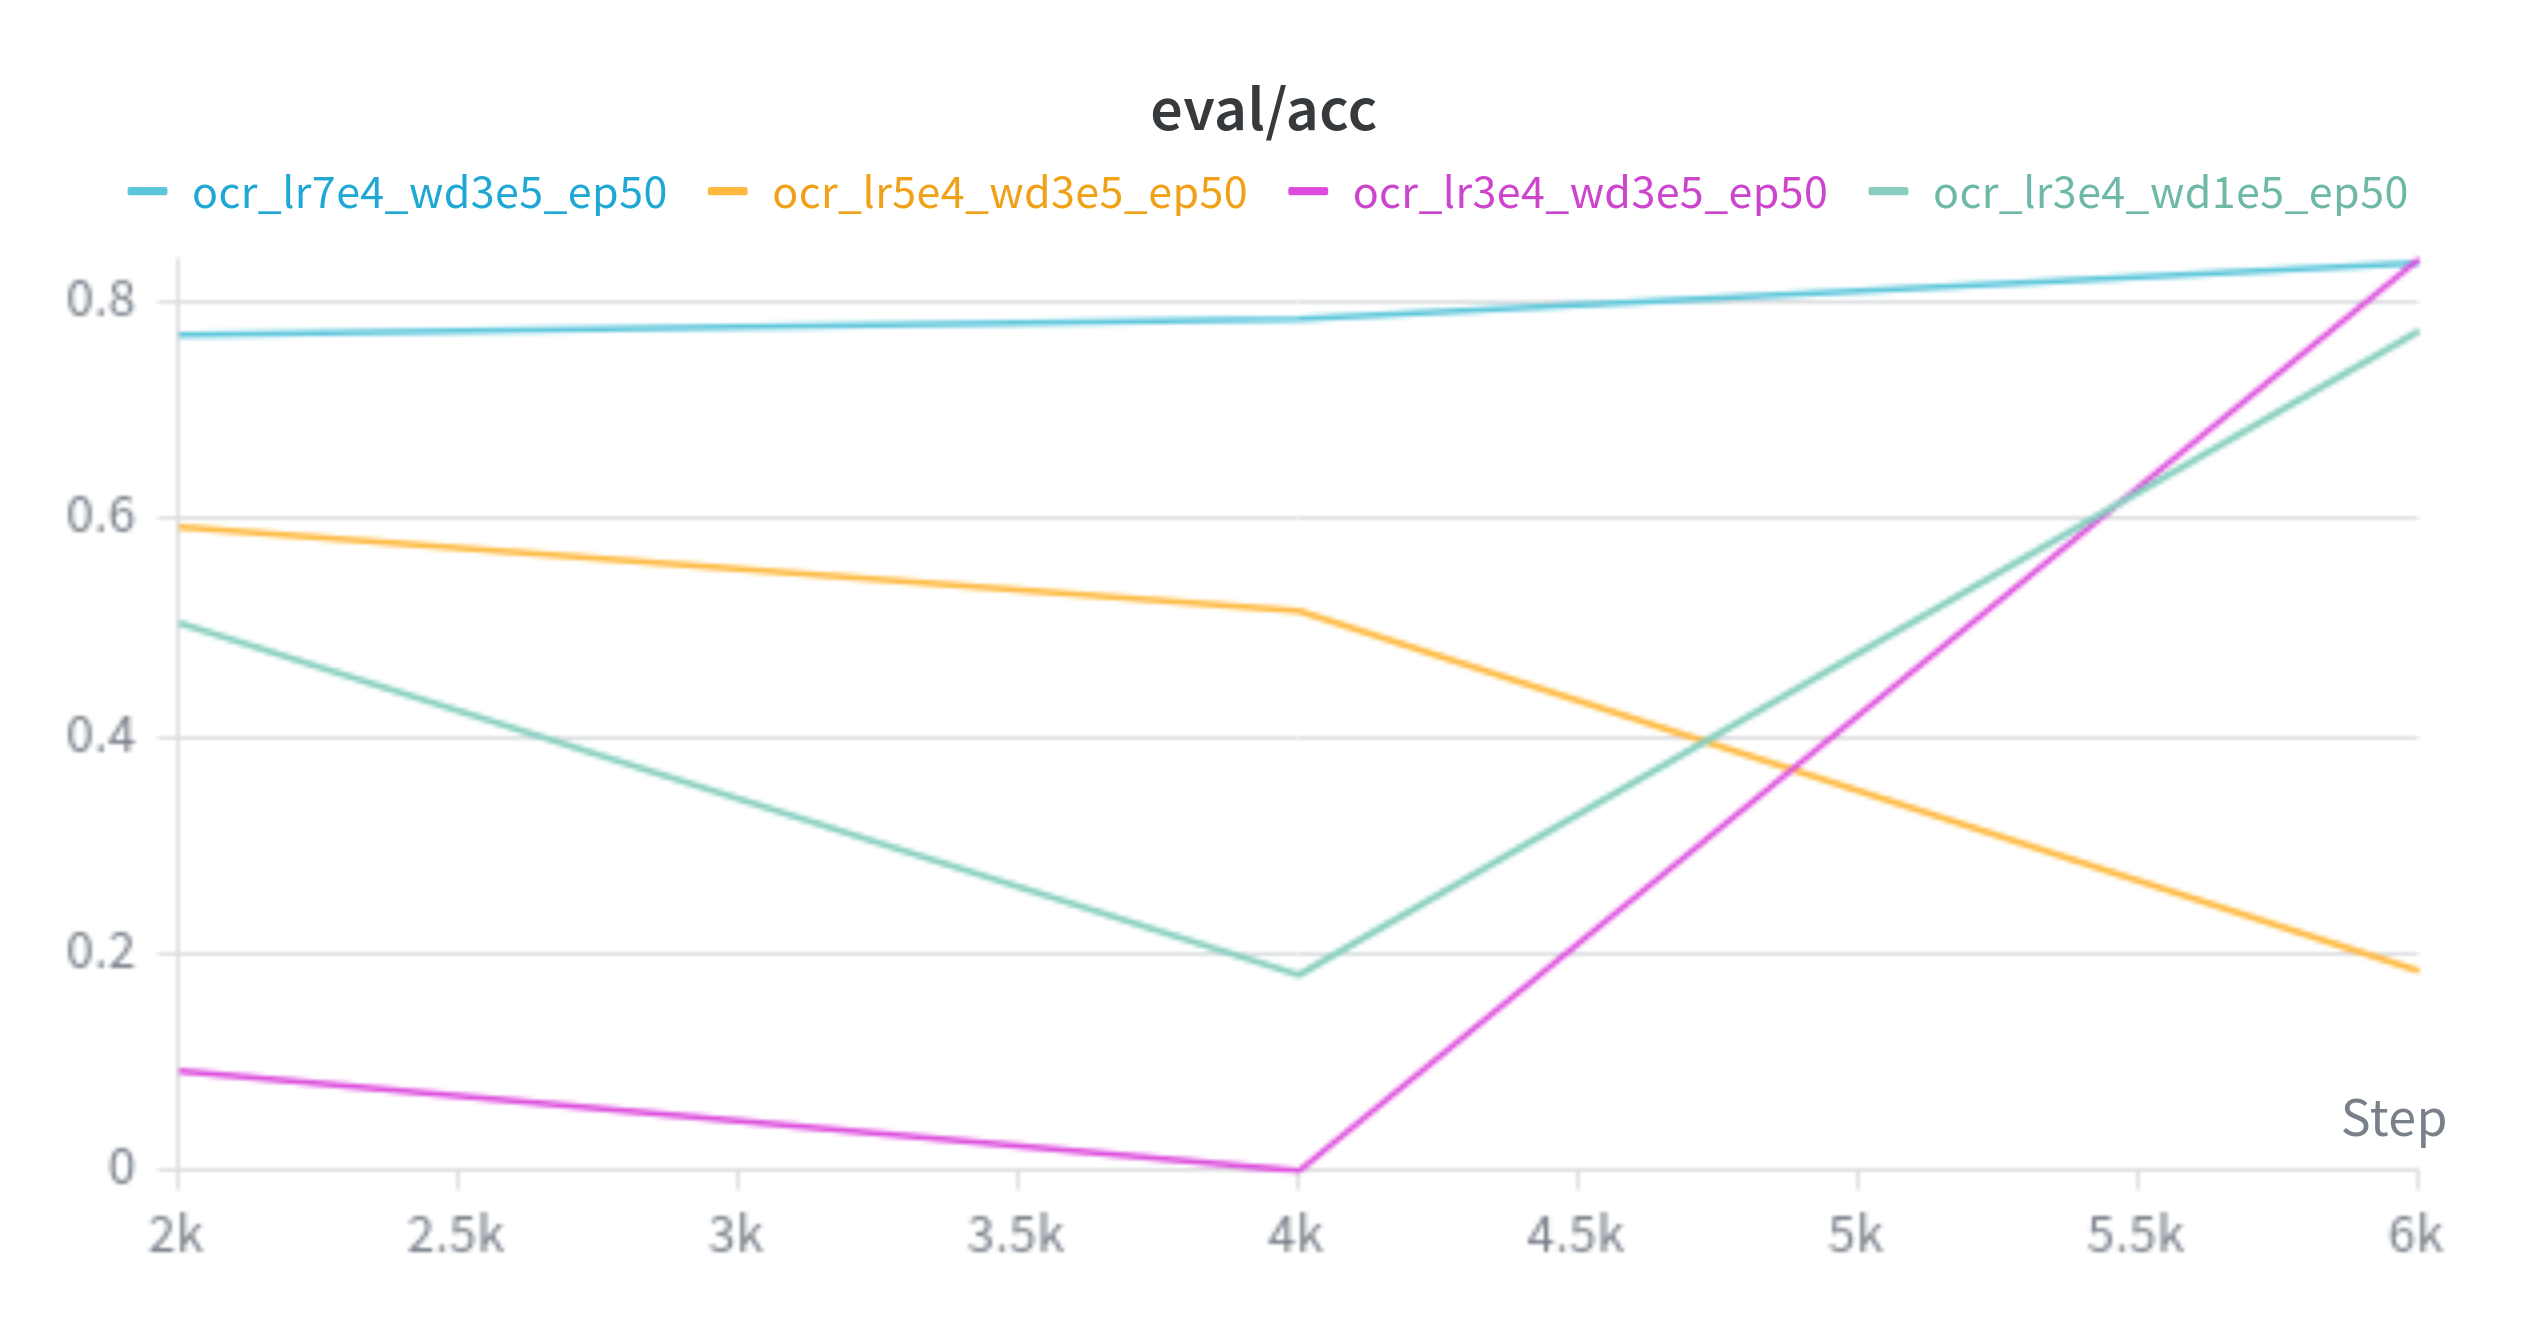
\includegraphics[width=0.82\textwidth]{figures/results/stage2_ocr_eval_acc.png}
    \caption{Stage 2 \gls{ocr} evaluation accuracy for the learning-rate and
    weight-decay sweep. The configuration with learning rate
    $3 \times 10^{-4}$ and weight decay $3 \times 10^{-5}$ achieved the best
    validation accuracy.}
    \label{fig:ocr_stage2_acc}
\end{figure}

\begin{figure}[htbp]
    \centering
    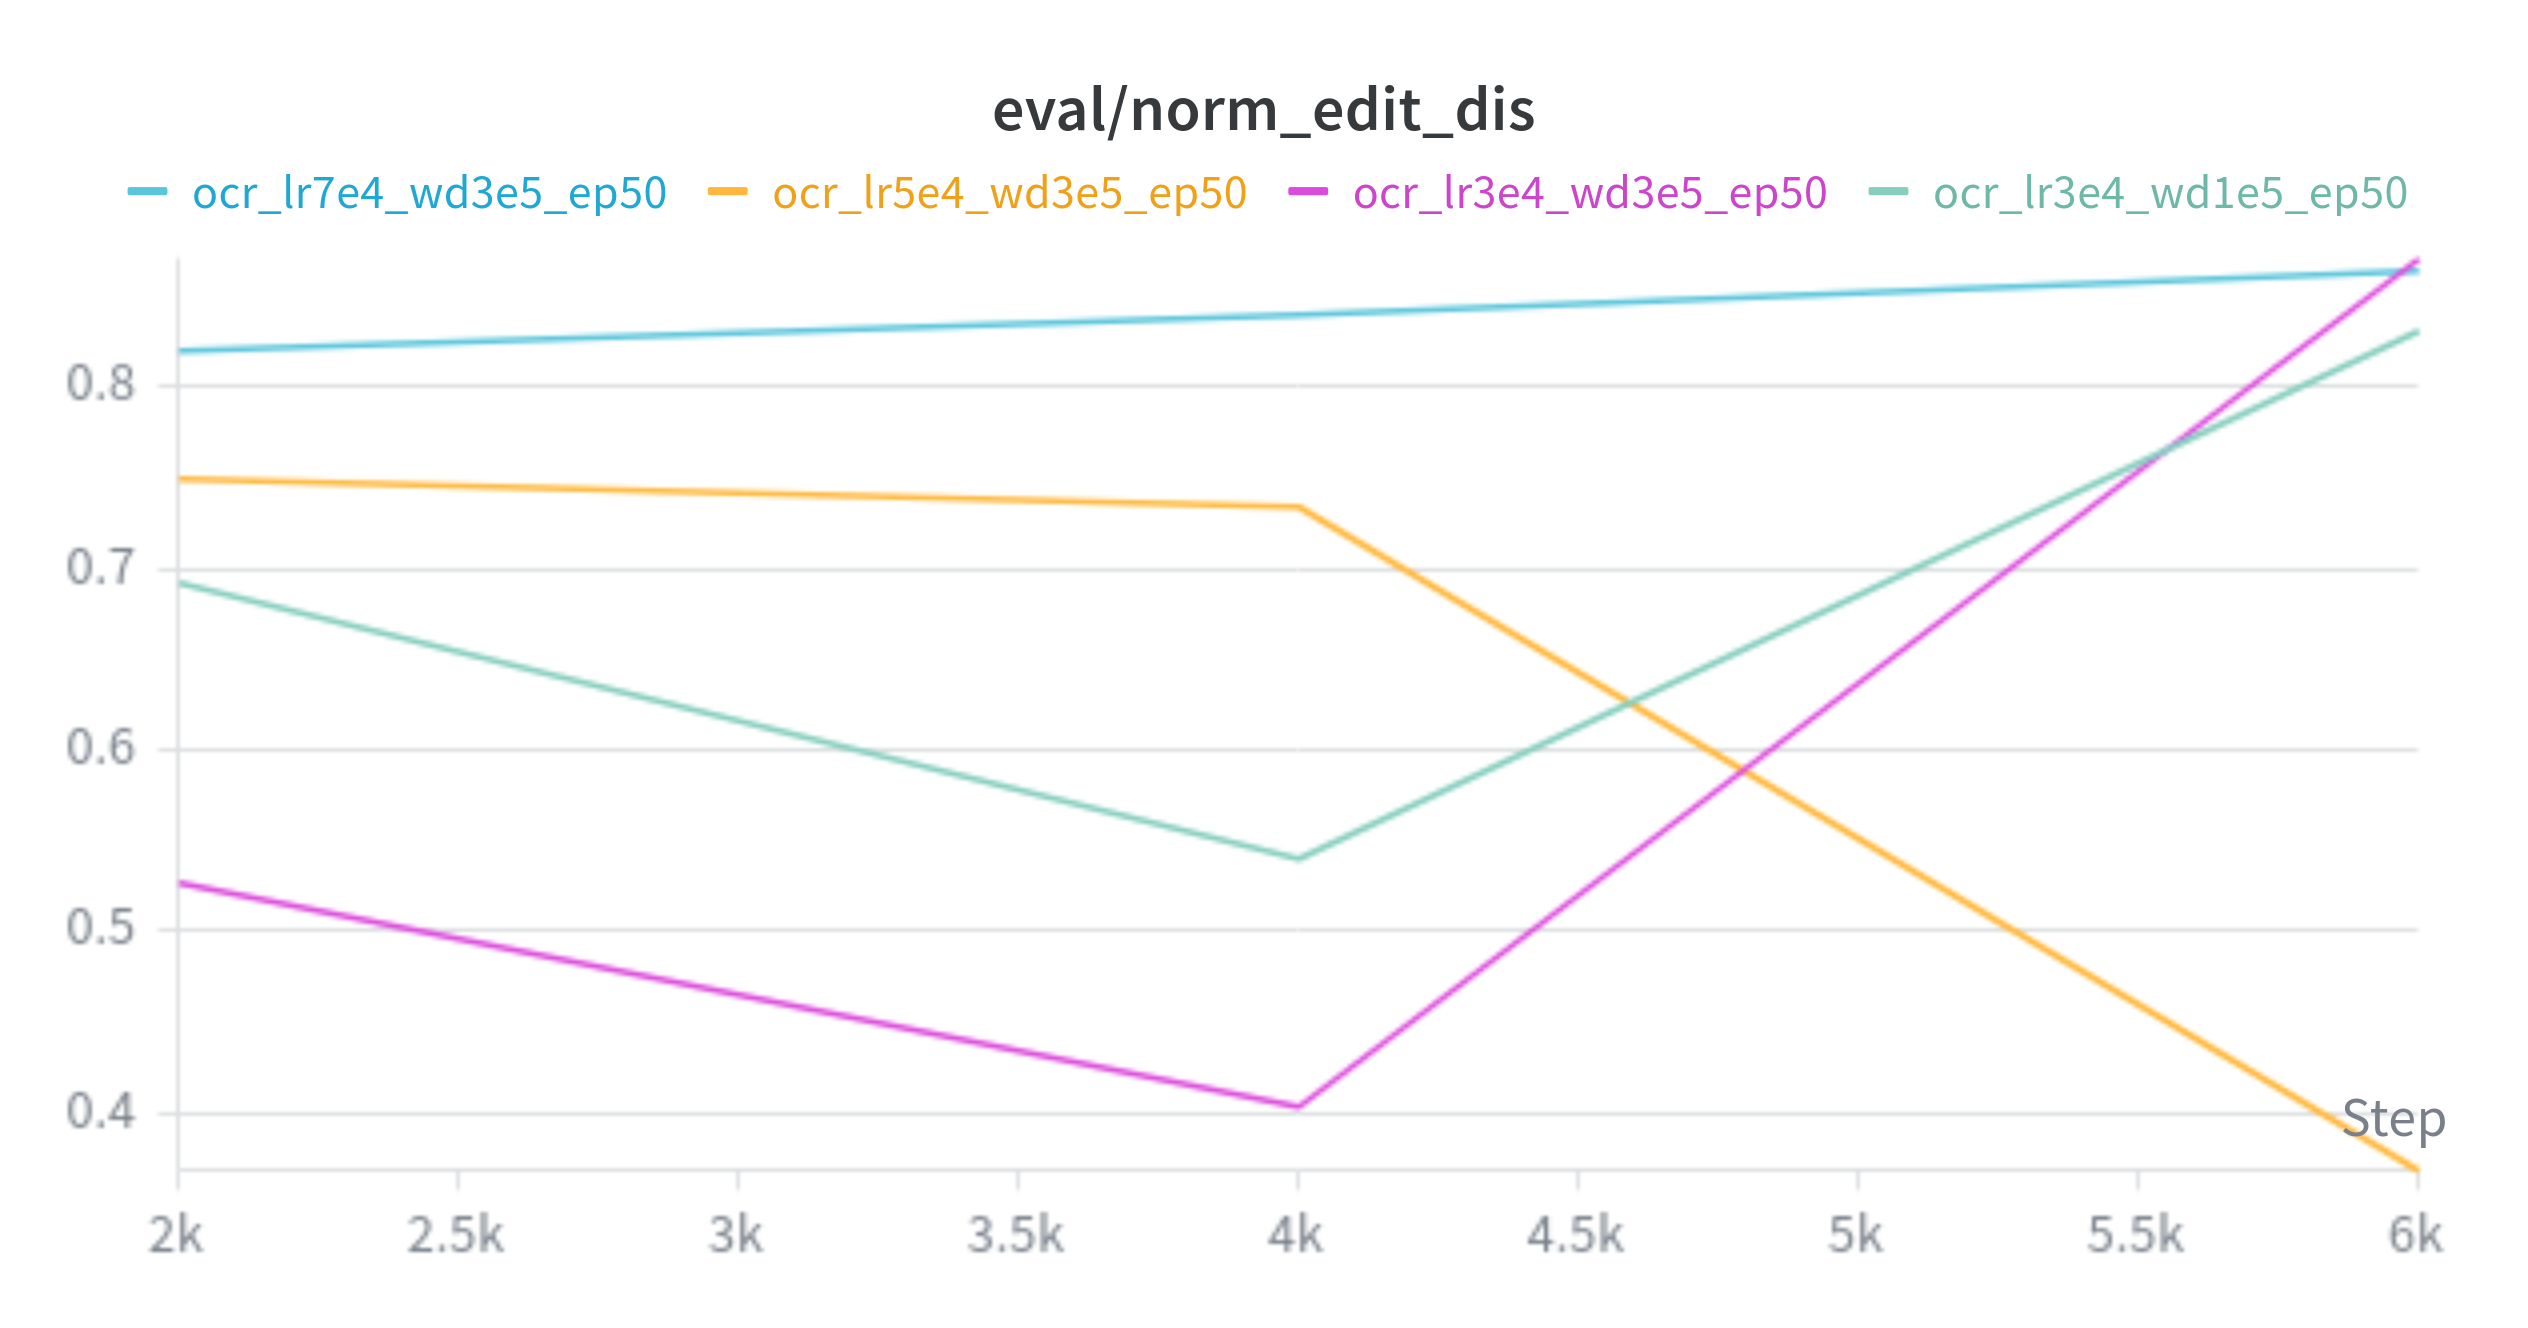
\includegraphics[width=0.82\textwidth]{figures/results/stage2_ocr_eval_norm_edit_dis.png}
    \caption{Stage 2 \gls{ocr} normalized edit distance for the learning-rate and
    weight-decay sweep. The best-performing configuration also achieved the
    highest normalized edit-distance score.}
    \label{fig:ocr_stage2_ned}
\end{figure}

\begin{table}[htbp]
    \centering
    \caption{Stage 2 \gls{ocr} hyperparameter sweep on the validation split.}
    \label{tab:ocr_stage2_results}
    \small
    \begin{tabular}{lcccc}
        \toprule
        Trial & Learning rate & Weight decay & Accuracy & Normalized edit distance \\
        \midrule
        lr3e4\_wd1e5\_ep50 & $3 \times 10^{-4}$ & $1 \times 10^{-5}$ & 0.77531 & 0.83148 \\
        lr3e4\_wd3e5\_ep50 & $3 \times 10^{-4}$ & $3 \times 10^{-5}$ & \textbf{0.84157} & \textbf{0.87098} \\
        lr5e4\_wd3e5\_ep50 & $5 \times 10^{-4}$ & $3 \times 10^{-5}$ & 0.59603 & 0.74899 \\
        lr7e4\_wd3e5\_ep50 & $7 \times 10^{-4}$ & $3 \times 10^{-5}$ & 0.83653 & 0.86546 \\
        \bottomrule
    \end{tabular}
\end{table}

\subsection{Final \gls{ocr} benchmark}

The final \gls{ocr} benchmark compared the original fine-tuned recognizer against the
best-performing stage-2 configuration on the held-out \gls{ocr} test set. The results
are shown in Table~\ref{tab:ocr_final_benchmark}. The stage-2 model outperformed
the initial \gls{ocr} model on both recognition-quality metrics. Test accuracy improved
from 0.81635 to 0.83486, while normalized edit distance improved from 0.85574 to
0.87190. In addition, the measured evaluation throughput increased slightly from
805.68 to 817.71 samples per second.

Taken together, these results show that the \gls{ocr} hyperparameter tuning process
produced a real improvement rather than only a validation-specific gain. Unlike
the \gls{yolo} tuning experiments, where better validation performance did not
translate into a better final test-set model, the \gls{ocr} stage-2 winner also
improved the held-out test benchmark. For this reason, the stage-2 best \gls{ocr} model
was selected as the final recognition candidate for later integration into the
complete perception pipeline.

\begin{table}[htbp]
    \centering
    \caption{Held-out \gls{ocr} test-set comparison between the initial recognizer and the selected stage-2 \gls{ocr} model.}
    \label{tab:ocr_final_benchmark}
    \small
    \begin{tabular}{lccc}
        \toprule
        Model & Accuracy & Normalized edit distance & Throughput (samples/s) \\
        \midrule
        Initial \glsentryshort{ocr} model & 0.81635 & 0.85574 & 805.68 \\
        Stage-2 best \glsentryshort{ocr} model & \textbf{0.83486} & \textbf{0.87190} & \textbf{817.71} \\
        \bottomrule
    \end{tabular}
\end{table}

\subsection{Model hardware optimization results}

As described in Chapter~3, the final \gls{yolo} and \gls{ocr} models were
exported to \gls{tensorrt} for optimized execution on the \gls{jetson} platform.
To verify the effect of this export step, a compact benchmark was performed on
the held-out test image \texttt{367.jpg}. For \gls{yolo}, the comparison used the
PyTorch checkpoint and the exported \gls{tensorrt} engine on the same full image.
For \gls{ocr}, the comparison used the Paddle inference model and the exported
\gls{tensorrt} engine on the five annotated button crops from the same image.

\begin{table}[htbp]
    \centering
    \caption{Single-image model hardware optimization benchmark on test image \texttt{367.jpg}. For \gls{ocr}, the reported latency is average time per single button crop.}
    \label{tab:model_hw_optimization}
    \small
    \begin{tabular}{lccc}
        \toprule
        Model stage & Baseline backend & \glsentryshort{tensorrt} backend & Speedup \\
        \midrule
        \glsentryshort{yolo} inference [ms/image] & 36.46 & 24.43 & 1.49$\times$ \\
        \glsentryshort{yolo} wall time [ms/image] & 64.19 & 64.52 & 1.00$\times$ \\
        \glsentryshort{ocr} latency [ms/crop] & 167.72 & 10.29 & 16.30$\times$ \\
        \bottomrule
    \end{tabular}
\end{table}

The \gls{yolo} result shows that \gls{tensorrt} reduced the forward-pass time
substantially, even though the total offline single-image wall time remained
almost unchanged because preprocessing and postprocessing still contributed a
large fraction of the runtime. The \gls{ocr} result is more direct: the
\gls{tensorrt} engine reduced average latency from 167.72~ms to 10.29~ms per
button crop while preserving the same accepted predictions on all five button
regions in the test image. These results support the use of \gls{tensorrt}
export as an important deployment optimization step before integrating the models
into the full \gls{ros2} pipeline.

\section{\Gls{ros2} pipeline performance}

After the final \gls{yolo} and \gls{ocr} models were exported to \gls{tensorrt}, the complete
perception stack was evaluated on the \gls{jetson} Orin Nano in its deployed \gls{ros2}
configuration. The purpose of these experiments was not to compare neural-network
accuracy, but to quantify the practical throughput of the integrated pipeline under
different runtime settings. The reported measurements correspond to the final
post-refactor pipeline in which ROI-local masks are published by the YOLO node and
full-image annotation reconstruction is performed only inside the \gls{adc} when
export is required. During these experiments, the Stereolabs ZED X camera was
launched with the \texttt{zedx} wrapper profile, which uses a native
\texttt{HD1200} grab mode at 30~Hz and publishes rectified color and depth data at
15~\gls{fps}. With the configured downscale factor of 2.0, the effective published
image resolution used by the perception pipeline was 960$\times$600 pixels.

Three final runtime scenarios were compared:
\begin{itemize}
    \item camera + \gls{yolo} + \gls{ocr} + \gls{adc},
    \item camera + \gls{yolo} + \gls{ocr} without collector and with \gls{ocr} uncapped, and
    \item camera + \gls{yolo} + \gls{ocr} without collector and with \gls{ocr} limited to four regions per message.
\end{itemize}

Table~\ref{tab:ros2_pipeline_fps} summarizes the resulting topic throughput. The
collector-enabled configuration sustained approximately 10~\gls{fps} while preserving
the full deployment data-collection path. When the collector was disabled and \gls{ocr}
was allowed to process all candidate regions, the end-to-end rate increased to
about 12.2~\gls{fps}. The best runtime-oriented configuration was obtained when \gls{ocr}
was capped to four regions per message, yielding approximately 13.1~\gls{fps}
end-to-end on the final \texttt{/button\_targets\_3d\_ocr} output topic. The
reported topic rates were measured with the standard \texttt{ros2 topic hz}
utility on the relevant output topics.

\begin{table}[htbp]
    \centering
    \caption{Final \gls{ros2} pipeline throughput on the \gls{jetson} Orin Nano after the ROI-mask refactor, measured with \texttt{ros2 topic hz}.}
    \label{tab:ros2_pipeline_fps}
    \small
    \begin{tabular}{lcc}
        \toprule
        Configuration & \texttt{/button\_targets\_3d} \gls{fps} & \texttt{/button\_targets\_3d\_ocr} \gls{fps} \\
        \midrule
        With collector & $\sim 10.0$ & $\sim 10.0$ \\
        No collector, \gls{ocr} uncapped & $\sim 12.15$ & $\sim 12.29$ \\
        No collector, \gls{ocr} capped to 4 ROIs & $\sim 13.14$--$13.47$ & $\sim 13.08$--$13.25$ \\
        \bottomrule
    \end{tabular}
\end{table}

The timing breakdown confirms that the final system bottleneck is not the \gls{tensorrt}
forward pass alone, but the combined cost of segmentation postprocessing, depth
estimation, and \gls{ocr} execution inside the live \gls{ros2} graph. Table~\ref{tab:ros2_pipeline_timing}
shows typical timing ranges of the \gls{yolo} and \gls{ocr} nodes for the three runtime
configurations. In collector mode, the YOLO node required approximately
81--91~ms per callback and the \gls{ocr} node 79--95~ms. Removing the collector while
keeping \gls{ocr} uncapped reduced the practical throughput penalty of data export but
still required roughly 11 processed \gls{ocr} regions per message, which kept \gls{ocr} total
time in the 77--102~ms range. Limiting \gls{ocr} to four regions reduced \gls{ocr} total time
to roughly 33--35~ms and allowed the complete pipeline to reach its best measured
throughput.

\begin{table}[htbp]
    \centering
    \caption{Typical node timing ranges for the final \gls{ros2} runtime experiments.}
    \label{tab:ros2_pipeline_timing}
    \small
    \resizebox{\textwidth}{!}{%
    \begin{tabular}{lcccc}
        \toprule
        Configuration & \glsentryshort{yolo} total [ms] & \glsentryshort{yolo} depth [ms] & \glsentryshort{ocr} total [ms] & \glsentryshort{ocr} processed ROIs \\
        \midrule
        With collector & $\sim 81$--$91$ & $\sim 3.6$--$6.6$ & $\sim 79$--$95$ & not capped \\
        No collector, \gls{ocr} uncapped & $\sim 78$--$99$ & $\sim 4$--$7$ & $\sim 77$--$102$ & $\sim 10.7$--$10.9$ \\
        No collector, \gls{ocr} capped to 4 ROIs & $\sim 70.4$--$77.8$ & $\sim 5.3$--$7.0$ & $\sim 33.0$--$35.2$ & $4.0$ \\
        \bottomrule
    \end{tabular}
    }
\end{table}

These results show that the integrated perception pipeline can operate at
deployment-relevant frame rates on the \gls{jetson} Orin Nano, provided that annotation
serialization is kept out of the real-time \gls{yolo} path and \gls{ocr} workload is bounded.
For runtime operation, the most effective configuration is the ROI-limited \gls{ocr}
setup without concurrent collection, which achieved approximately 13.1~\gls{fps}.
For deployment sessions that must simultaneously gather new training data, the
collector-enabled configuration remains practical at approximately 10~\gls{fps},
which is sufficient to preserve the full adaptive data-collection loop described in
Chapter~\ref{ch:methodology}.
